% By default, output is produced that is geared toward generating a PDF 
% version optimized for viewing on an electronic display, including 
% hyperlinks within the PDF.
 
% E.g. to process a thesis called "mythesis.tex" based on this template, run:

% pdflatex mythesis	-- first pass of the pdflatex processor
% bibtex mythesis	-- generates bibliography from .bib data file(s) 
%(might as well need MakeIndex)
% pdflatex mythesis	-- fixes cross-references, bibliographic references, etc
% pdflatex mythesis	-- fixes cross-references, bibliographic references, etc

% If you use the recommended LaTeX editor, Texmaker, you would open the mythesis.tex
% file, then click the pdflatex button. Then run BibTeX (under the Tools menu).
% Then click the pdflatex button two more times. If you have an index as well,
% you'll need to run MakeIndex from the Tools menu as well, before running pdflatex
% the last two times.

% N.B. The "pdftex" program allows graphics in the following formats to be
% included with the "\includegraphics" command: PNG, PDF, JPEG, TIFF
% Tip 1: Generate your figures and photos in the size you want them to appear
% in your thesis, rather than scaling them with \includegraphics options.
% Tip 2: Any drawings you do should be in scalable vector graphic formats:
% SVG, PNG, WMF, EPS and then converted to PNG or PDF, so they are scalable in
% the final PDF as well.
% Tip 3: Photographs should be cropped and compressed so as not to be too large.

% To create a PDF output that is optimized for double-sided printing: 
%
% 1) comment-out the \documentclass statement in the preamble below, and
% un-comment the second \documentclass line.
%
% 2) change the value assigned below to the boolean variable
% "PrintVersion" from "false" to "true".

% --------------------- Start of Document Preamble -----------------------

% Specify the document class, default style attributes, and page dimensions
% For hyperlinked PDF, suitable for viewing on a computer, use this:
\documentclass[letterpaper,12pt,titlepage,oneside,final]{book}
 
% For PDF, suitable for double-sided printing, change the PrintVersion variable below
% to "true" and use this \documentclass line instead of the one above:
%\documentclass[letterpaper,12pt,titlepage,openright,twoside,final]{book}

% Some LaTeX commands I define for my own nomenclature.
% If you have to, it's better to change nomenclature once here than in a 
% million places throughout your thesis!
\newcommand{\package}[1]{\textbf{#1}} % package names in bold text
\newcommand{\cmmd}[1]{\textbackslash\texttt{#1}} % command name in tt font 
\newcommand{\href}[1]{#1} % does nothing, but defines the command so the
    % print-optimized version will ignore \href tags (redefined by hyperref pkg).
%\newcommand{\texorpdfstring}[2]{#1} % does nothing, but defines the command
% Anything defined here may be redefined by packages added below...

% This package allows if-then-else control structures.
\usepackage{ifthen}
\newboolean{PrintVersion}
\setboolean{PrintVersion}{false} 
% CHANGE THIS VALUE TO "true" as necessary, to improve printed results for hard copies
% by overriding some options of the hyperref package below.

%\usepackage{nomencl} % For a nomenclature (optional; available from ctan.org)
\usepackage{amsmath,amssymb,amstext} % Lots of math symbols and environments
\usepackage[pdftex]{graphicx} % For including graphics N.B. pdftex graphics driver 
\usepackage[bottom]{footmisc}
\usepackage{float}
\usepackage{subcaption}
\usepackage{setspace}
\usepackage[utf8]{inputenc}
\DeclareUnicodeCharacter{2009}{\,}
\usepackage [english]{babel}
\usepackage [autostyle, english = american]{csquotes}
\MakeOuterQuote{"}
\usepackage{tikz,pgfplots}
\usetikzlibrary{calc}
\usepackage{romannum}
\usepackage{siunitx}
\usepackage{chemfig}
\usepackage[numbers]{natbib}
%\usepackage{url}

% N.B. HYPERREF MUST BE THE LAST PACKAGE LOADED; ADD ADDITIONAL PKGS ABOVE
\usepackage[pdftex,letterpaper=true,pagebackref=false]{hyperref} % with basic options
		% N.B. pagebackref=true provides links back from the References to the body text. This can cause trouble for printing.
\hypersetup{
    plainpages=false,       % needed if Roman numbers in frontpages
    pdfpagelabels=true,     % adds page number as label in Acrobat's page count
    bookmarks=true,         % show bookmarks bar?
    unicode=false,          % non-Latin characters in Acrobat’s bookmarks
    pdftoolbar=true,        % show Acrobat’s toolbar?
    pdfmenubar=true,        % show Acrobat’s menu?
    pdffitwindow=false,     % window fit to page when opened
    pdfstartview={FitH},    % fits the width of the page to the window
    pdftitle={Junjie Yin 2018},    % title: CHANGE THIS TEXT!
    pdfauthor={Junjie Yin},    % author: CHANGE THIS TEXT! and uncomment this line
%    pdfsubject={Subject},  % subject: CHANGE THIS TEXT! and uncomment this line
%    pdfkeywords={keyword1} {key2} {key3}, % list of keywords, and uncomment this line if desired
    pdfnewwindow=true,      % links in new window
    colorlinks=true,        % false: boxed links; true: colored links
    linkcolor=blue,         % color of internal links
    citecolor=green,        % color of links to bibliography
    filecolor=magenta,      % color of file links
    urlcolor=cyan           % color of external links
}
\ifthenelse{\boolean{PrintVersion}}{   % for improved print quality, change some hyperref options
\hypersetup{	% override some previously defined hyperref options
%    colorlinks,%
    citecolor=black,%
    filecolor=black,%
    linkcolor=black,%
    urlcolor=black}
}{} % end of ifthenelse (no else)

% Setting up the page margins...
% uWaterloo thesis requirements specify a minimum of 1 inch (72pt) margin at the
% top, bottom, and outside page edges and a 1.125 in. (81pt) gutter
% margin (on binding side). While this is not an issue for electronic
% viewing, a PDF may be printed, and so we have the same page layout for
% both printed and electronic versions, we leave the gutter margin in.
% Set margins to minimum permitted by uWaterloo thesis regulations:
\setlength{\marginparwidth}{0pt} % width of margin notes
% N.B. If margin notes are used, you must adjust \textwidth, \marginparwidth
% and \marginparsep so that the space left between the margin notes and page
% edge is less than 15 mm (0.6 in.)
\setlength{\marginparsep}{0pt} % width of space between body text and margin notes
\setlength{\evensidemargin}{0.125in} % Adds 1/8 in. to binding side of all 
% even-numbered pages when the "twoside" printing option is selected
\setlength{\oddsidemargin}{0.125in} % Adds 1/8 in. to the left of all pages
% when "oneside" printing is selected, and to the left of all odd-numbered
% pages when "twoside" printing is selected
\setlength{\textwidth}{6.375in} % assuming US letter paper (8.5 in. x 11 in.) and 
% side margins as above
\raggedbottom

% The following statement specifies the amount of space between
% paragraphs. Other reasonable specifications are \bigskipamount and \smallskipamount.
\setlength{\parskip}{\medskipamount}

% The following statement controls the line spacing.  The default
% spacing corresponds to good typographic conventions and only slight
% changes (e.g., perhaps "1.2"), if any, should be made.
\renewcommand{\baselinestretch}{1} % this is the default line space setting

% By default, each chapter will start on a recto (right-hand side)
% page.  We also force each section of the front pages to start on 
% a recto page by inserting \cleardoublepage commands.
% In many cases, this will require that the verso page be
% blank and, while it should be counted, a page number should not be
% printed.  The following statements ensure a page number is not
% printed on an otherwise blank verso page.
\let\origdoublepage\cleardoublepage
\newcommand{\clearemptydoublepage}{%
  \clearpage{\pagestyle{empty}\origdoublepage}}
\let\cleardoublepage\clearemptydoublepage

\begin{document}

% T I T L E   P A G E
% -------------------

\pagestyle{empty}
\pagenumbering{roman}

\begin{titlepage}
        \begin{center}
        \vspace*{1.0cm}

        \Huge
        {\bf Production and Analysis of Highly Monodisperse Oligomeric Poly(Ethylene Oxide) }

        \vspace*{1.0cm}

        \normalsize
        by \\

        \vspace*{1.0cm}

        \Large
        Junjie Yin \\

        \vspace*{3.0cm}

        \normalsize
        A thesis \\
        presented to the University of Waterloo \\ 
        in fulfillment of the \\
        thesis requirement for the degree of \\
        Master of Science \\
        in \\
        Physics (Nanotechnology)\\

        \vspace*{2.0cm}

        Waterloo, Ontario, Canada, 2018 \\

        \vspace*{1.0cm}

        \copyright\ Junjie Yin 2018 \\
        \end{center}
\end{titlepage}

% The rest of the front pages should contain no headers and be numbered using Roman numerals starting with `ii'
\pagestyle{plain}
\setcounter{page}{2}

\cleardoublepage % Ends the current page and causes all figures and tables that have so far appeared in the input to be printed.
% In a two-sided printing style, it also makes the next page a right-hand (odd-numbered) page, producing a blank page if necessary.
 
\doublespacing

% D E C L A R A T I O N   P A G E
% -------------------------------
  % The following is the sample Delaration Page as provided by the GSO
  % December 13th, 2006.  It is designed for an electronic thesis.
  \noindent
I hereby declare that I am the sole author of this thesis. This is a true copy of the thesis, including any required final revisions, as accepted by my examiners.

  \bigskip
  
  \noindent
I understand that my thesis may be made electronically available to the public.

\cleardoublepage
%\newpage

% A B S T R A C T
% ---------------

\begin{center}\textbf{Abstract}\end{center}

Poly(Ethylene Oxide), along with Poly(Ethylene) and n-alkanes, are the most intensively studied polymers in terms of crystallization, because of their linear structure. In this thesis, we investigate three different aspects of PEO oligomers, and the chapters are organized in a self-contained fashion, with a general introduction and a brief conclusion. We introduce the production of highly monodisperse PEO oligomers, and the analysis of their crystallization and melting behaviors. Through evaporative purification, we have been able to purify low molecular weight PEO, and achieve a polydispersity index six times better than the neat commercial sample, measured by mass spectroscopy. Melting temperatures are obtained using differential scanning calorimetry. Based on Gibbs Thomson relation, we claim that during crystallization, purified PEO samples can form crystal lamellae not only with extended chains, but also with once-folded chains, which is normally not expected for polymers with such short chain lengths. 3.5 monomers are required to complete each fold, as suggested by the fitting of Gibbs Thomson curve. The fact that we are able to control the melting temperature validates our chain-folding model of folded and extended chains.

\cleardoublepage
%\newpage

% A C K N O W L E D G E M E N T S
% -------------------------------

% T A B L E   O F   C O N T E N T S
% ---------------------------------
% To define the depth that the table of contents goes, set the following in the preamble:
%\setcounter{tocdepth}{1} % Show sections
%\setcounter{tocdepth}{2} % + subsections
%\setcounter{tocdepth}{3} % + subsubsections
%\setcounter{tocdepth}{4} % + paragraphs
%\setcounter{tocdepth}{5} % + subparagraphs

\renewcommand\contentsname{Table of Contents}
\tableofcontents
\cleardoublepage
\phantomsection
%\newpage

% L I S T   O F   T A B L E S
% ---------------------------
%\addcontentsline{toc}{chapter}{List of Tables}
%\listoftables
%\cleardoublepage
%\phantomsection		% allows hyperref to link to the correct page
%\newpage

% L I S T   O F   F I G U R E S
% -----------------------------
\addcontentsline{toc}{chapter}{List of Figures}
\listoffigures
\cleardoublepage
\phantomsection		% allows hyperref to link to the correct page
%\newpage

% L I S T   O F   S Y M B O L S
% -----------------------------
% To include a Nomenclature section
% \addcontentsline{toc}{chapter}{\textbf{Nomenclature}}
% \renewcommand{\nomname}{Nomenclature}
% \printglossary
% \cleardoublepage
% \phantomsection % allows hyperref to link to the correct page
% \newpage

% Change page numbering back to Arabic numerals
\pagenumbering{arabic}

 

\chapter{Introduction}
\graphicspath{{./introduction/graphs/}}

\onehalfspacing
%======================================================================
\section{Polymer}

Polymers are large molecules that consist of repeating units, called monomers. The number of monomers that a polymer contains is defined as its degree of polymerization, $N$. Thus the molecular weight of a polymer is $M = NM_{mon}$, where $M_{mon}$ is the molecular weight of a monomer. Typically, the backbone of a polymer is composed of carbon atoms connected to each other by covalent bonds. Polymers that contain only one type of monomers are called homopolymers, while those containing more than one type are called heteropolymers \cite{Rubinstein2003}. 

Polymer samples normally exist as a collection of polymer molecules with unequal molecular weights, hence the average molecular weight of the entire sample is described as either number average molecular weight, $M_{n}$, or weight average molecular weight, $M_{w}$: 

\begin{equation}
\label{Mn}
M_{n} = \dfrac{\sum N_{i}M_{i}}{N_{i}}
\end{equation}

\begin{equation}
\label{Mw}
M_{w} = \dfrac{\sum N_{i}M_{i}^{2}}{N_{i}M_{i}}
\end{equation}

where $M_{i}$ is the molecular weight of a polymer chain, and $N_{i}$ is the number of polymer chains with molecular weight $M_{i}$. On both sides of $M_{n}$, there are equal numbers of polymers, while on both sides of $M_{w}$, there are equal weights of polymers. 

Polydispersity index is defined by the ratio of $M_{w}$ to $M_{n}$, and it describes how broad the distribution of molecular weight is. If all the polymers have the same molecular weight, PDI is equal to 1, and the sample is called monodisperse. The larger the PDI is, the broader the molecular weight distribution is, which is normally undesirable. For an intuitive sense of PDI, here is an example. A sample contains half, by number, of polymers with molecular weight 1000, and the other half with molecular weight 2000. $M_{n}$ of this sample is calculated to be 1500, and $M_{w}$ is 1667. Thus PDI of this sample is 1.11, which appears decent, but the corresponding sample is far from pure. In real cases the polymers are more likely to have a Gaussian distribution of different molecular weights rather than shown in this particular example, but this calculation gives us an idea of how PDI could be hiding the actual composition of a polymer sample.

\section{Polymerization}

Synthesized polymers contain a distribution of different molecular weights. Even the most monodisperse synthetic polymers have a polydispersity index (PDI) of about 1.01 \cite{Thakur2016}, which still contain many different $N$ values. This fact is closely related to the process of producing synthetic polymers, polymerization.

Polymerization is the process of connecting monomers together onto a polymer chain. This process could be achieved through different methods. Common methods include step-growth polymerization, chain-growth polymerization, and living anionic polymerization, which is a special case of chain-growth. 

Step-growth polymerization refers to the process in which stepwise reactions among functional groups of monomers form polymers. Typical polymers produced by step-growth include polyamide (nylon), polyester, and polyether \cite{Carraher2003a}. 

Chain-growth polymerization refers to the process in which unsaturated monomers are added onto the active sites of a growing polymer successively. Typical polymers produced by chain-growth include polyethylene, polypropylene, and polyvinyl chloride \cite{YOUNG2017}. 

Being a special case of chain-growth, living polymerization is a process in which the termination step of the polymer growth is eliminated, and the rate of chain initiation is much larger than chain propagation, making the polymer growth easier to control. Living anionic polymerization, with anionic propagating species, is one of the most common methods of living polymerization \cite{Halasa1981}. 

Based on different mechanisms, these methods lead to different polydispersity indices. The typical PDI that step-growth leads to is around 2, and for common chain-growth such as free radical polymerization, it is 1.2 $\sim$ 1.5. Living anionic polymerization normally leads to a PDI less than 1.2, which could even reach a number very close to 1, provided with proper conditions \cite{Dotson1995}.

\section{Poly(Ethylene Oxide)}

Poly(Ethylene Oxide), also known as Poly(Ethylene Glycol) or Poly(OxyEthylene), is a polymer with the repeating unit:

\begin{center}
\def\setpolymerdelim#1#2{%
	\def\delimleft{#1}%
	\def\delimright{#2}%
}

\def\makebraces[#1,#2]#3#4#5{%
	\edef\delimhalfdim{\the\dimexpr(#1+#2)/2}%
	\edef\delimvshift{\the\dimexpr(#1-#2)/2}%
	\chemmove{%
		\node[at=(#4),yshift=(\delimvshift)]%
		{$\expandafter\left\delimleft\vrule height \delimhalfdim depth \delimhalfdim width 0pt\right.$};%
		\node[at=(#5),yshift=(\delimvshift)]%
		{$\left.\vrule height \delimhalfdim depth \delimhalfdim width 0pt \expandafter\right\delimright_{\rlap{#3}}$};%
	}%
}

\setpolymerdelim()

\chemfig{\vphantom{CH_2}-[@{op,.75}]CH_2-CH_2-O-[@{cl,0.25}]}
\makebraces[5pt,5pt]{\!\!n}{op}{cl}
\end{center}

PEO has various architectures, including linear, branched, star and comb, and the most widely used type in industry, especially for high molecular weights, is linear PEO. It is soluble in water, acetone, alcohols, benzene, dichloromethane, chloroform, ethanol, methanol, etc., depending on its molecular weight \cite{Brady2017}. 

Low molecular weight PEO is liquid at room temperature, and its melting point increases with molecular weight, with an upper limit of \SI{68.9}{\celsius} \cite{Buckley1975}, which is the predicted melting temperature of PEO with infinitely larger molecular weight.

PEO based materials have advantages such as non-toxicity, low cost, and electrochemical stability \cite{Xue2015}. Therefore they have a wide range of applications in fields including biology, chemistry, and medicine. Because of its excellent ion conductivity, one of the most promising applications is to act as electrolyte material in lithium ion batteries \cite{Croce1998}. However, it is the amorphous phase in PEO that contributes to ion conductivity, while the linear structure of PEO leads to high crystallinity, which restrains ion transportation especially at low temperatures. Thus, researches on PEO crystallization are of great importance.

In this research, the PEO sample purchased from Sigma Aldrich, Inc. has an average $M_{n}$ of 600, which appears as waxy solid at room temperature. It has the following chemical structure, with both ends being hydroxy group.

\begin{figure}[H]
	\center
	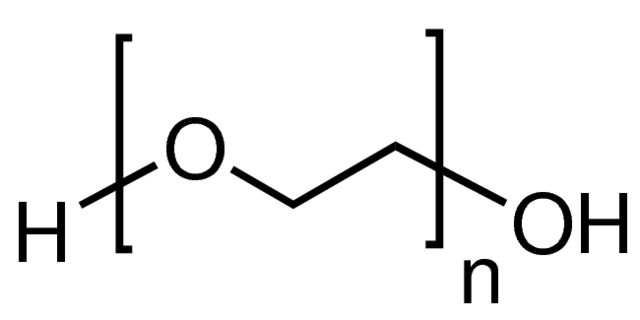
\includegraphics[width=0.3\linewidth]{PEO600}
	\caption[Chemical structure of PEO sample with average $M_{n}$ of 600.]{Chemical structure of PEO sample with average $M_{n}$ of 600 \cite{Sigma-Aldrich2018}.}
	\label{fig:PEO600}
\end{figure}

\section{Importance of $N$}

The degree of polymerization N has an important effect on many properties of polymers. According to Flory-Huggins equation \cite{Rubinstein2003}: 

\begin{equation}
\label{eqn_free energy}
\Delta F_{mix} = kT [\dfrac{\phi}{N} \ln \phi + (1 - \phi) \ln (1 - \phi) + \chi \phi (1 - \phi)]
\end{equation}

\noindent
where the free energy of mixing a polymer with a solvent, $\Delta F_{mix}$, is dependent on $N$. Therefore different $N$'s cause different solubilities. 

Another property that $N$ influences is glass transition temperature $T_{g}$. Glass transition is one of the most crucial phase transitions in polymer science, which refers to the temperature at which the free volume available for molecular motions achieves a minimum. According to Flory-Fox equation \cite{Fox1950a}:

\begin{equation}
\label{eqn_fox-flory}
T_{g} = T_{g,\infty} - \dfrac{K}{M_{n}}
\end{equation}

\noindent
$T_{g}$ is dependent on $M_{n}$, which is directly determined by $N$.

Polymer crystallization is also affected by $N$. One example is atactic polystyrene (aPS). Atactic indicates that the phenyl groups are randomly oriented along the chain. Therefore, crystallization is less preferred for aPS, and thus it has been described as a non-crystal. However, using atomic force microscope (AFM), Yu Chai \textit{et al} \cite{Chai2016} discovered that aPS with $M_{w}$ 600 $g/mol$, which corresponds to a very low $N$, does crystallize. This indicates that $N$ has an unpredictable effect on polymer crystallization. To explore this effect, this research examines the crystallization of PEO oligomers, as a special example.

\section{Polymer crystallization}

Crystallization of large molecules has long been a research topic intensively studied, yet with numerous questions unsolved and mechanisms to be understood. The main factor that causes the essential difference in polymer crystallization and crystallization of a regular small molecule is the long chain nature of a polymer. Long chains could easily get entangled, which prevent themselves from being aligned in order in the crystalline lattice. However, crystallization is still possible in certain polymers, with a much different structure than regular crystals.

In this thesis, PEO is our subject of crystallization study. As a matter fact, this linear polymer has many properties in common with n-alkanes, therefore studies on n-alkanes crystallization could also give us insights on our research. For n-alkanes crystallization from melt, investigations have been focus on aspects including crystal structure, chain conformations, nucleation and growth mechanisms, etc. Conformation of n-alkane chains in the crystal include both extended chains and folding of chains \cite{Organ1996,Alamo1993}, where the number of folds depend on chain lengths, crystallization conditions, etc. Nulceation and growth rates of n-alkanes crystals have also been investigated, and most studies are based on experimental methods including X-ray diffraction (XRD), small angle X-ray spectroscopy (SAXS), infrared spectroscopy, optical microscopy, and electron microscopy, as well as computer simulation methods such as molecular dynamics (MD) simulations \cite{Anwar2013,Yamamoto2016}.

In Chapter \ref{chap_analysis}, a more detailed review on polymer crystallization and PEO crystallizaiton in particular is provided, mainly focusing on the thermodynamics and crystal structure. In Chapter \ref{chap_growth}, polymer crystallization kinetics, including nucleation and crystal growth mechanisms are reviewed.


\chapter{Evaporative purification}
\graphicspath{{./evaporation/graphs/}}

In order to study the effects of $N$, the first thing needed is to obtain very monodisperse samples with different $N$ values. This has been achieved through an evaporative purification technique, which has been practised on low molecular weight polystyrene, and proved to be an efficient way to obtain highly monodisperse polymers \cite{Zhu2017a}.

\section{Vapour pressure of PEO oligomers}

For a particular polymer, as its $N$ decreases, its vapour pressure increases, and for polymers with small enough $N$ values, their vapour pressure could be significant at high temperatures (lower than their thermal degradation temperature). This fact potentially allows one to separate polymer components with different $N$ values, by applying an evaporation method similar to distillation.

To examine the feasibility of separating components through evaporation, it is a good idea to first look at their vapour pressures. Unfortunately, there are few data of vapour pressure of pure PEO \cite{Krieger2018}, either from calculation or experimental measurements. Therefore, we applied a theoretical model to calculate the vapour pressures of low molecular weight PEO.

Sanchez and Lacombe's Lattice-Fluid Model \cite{Sanchez1976} describes a fluid using only three molecular parameters, and provides a method to calculate the relation between vapour pressure and temperature for a given $N$ value. These three parameters for PEO could be found in the literature \cite{Rodgers1993}.

In this model, Gibbs free energy G is a function of mass density $\rho$:

\begin{equation}
G = - \rho + P\nu + T[(\nu - 1)\ln(1 - \rho) + \dfrac{1}{r}\ln(\rho/\omega)]  \label{eqn_Gvsrho}
\end{equation}

\noindent
where $\rho$ is reduced density, $P$ is reduced pressure, $\nu$ is reduced volume, $T$ is reduced temperature, $r$ is the number of monomers in a polymer molecule, and $\omega = \delta r/\sigma e^{r-1}$ ($\delta$ is the flexible parameter, and $\sigma$ is the symmetry number). For a specific $N$ at given pressure and temperature, G could be plotted as a function of $\rho$ as shown below.

\begin{figure}[H]
\center
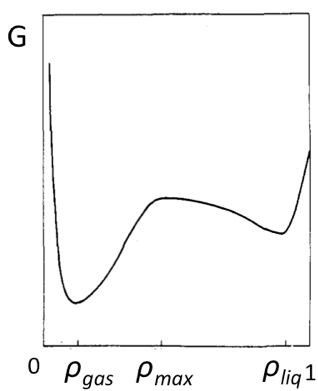
\includegraphics[width=0.2\linewidth]{Gvsrho}
\caption[Gibbs free energy vs mass density, where a liquid phase is metastable with respect to the vapour phase]{Gibbs free energy vs mass density, where a liquid phase is metastable with respect to the vapour phase. Figure source: "An elementary molecular theory of classical fluids. Pure
fluids" by Isaac C. Sanchez \textit{et al}, \textit{J. Phys. Chem.}, 80(21):2352-2362, 1976 \cite{Sanchez1976}.}
\label{fig:Gvsrho}
\end{figure}

The curve has two local minima. The first minimum represents the gas phase, with lower mass density, and the second minimum represents the liquid phase, with higher mass density. By tuning pressure or temperature, the two minima can be adjusted to be equal. This means the system has equal probability to be in the state of either gas or liquid. At a given temperature, there exists only one pressure that satisfies this equality, and this pressure and temperature are defined as the saturation pressure and temperature. The locus of all the saturation points represents the saturation/coexistence line, which is in fact the curve of vapour pressure as a function of temperature.

Solving Equation \ref{eqn_Gvsrho} and applying the three molecular parameters found in literature, we were able to calculate the vapour pressure curve for each $N$ value of PEO oligomers. The results are shown in the plot below, and note that each curve has been generated from 10-20 calculated points.

\begin{figure}[H]
\center
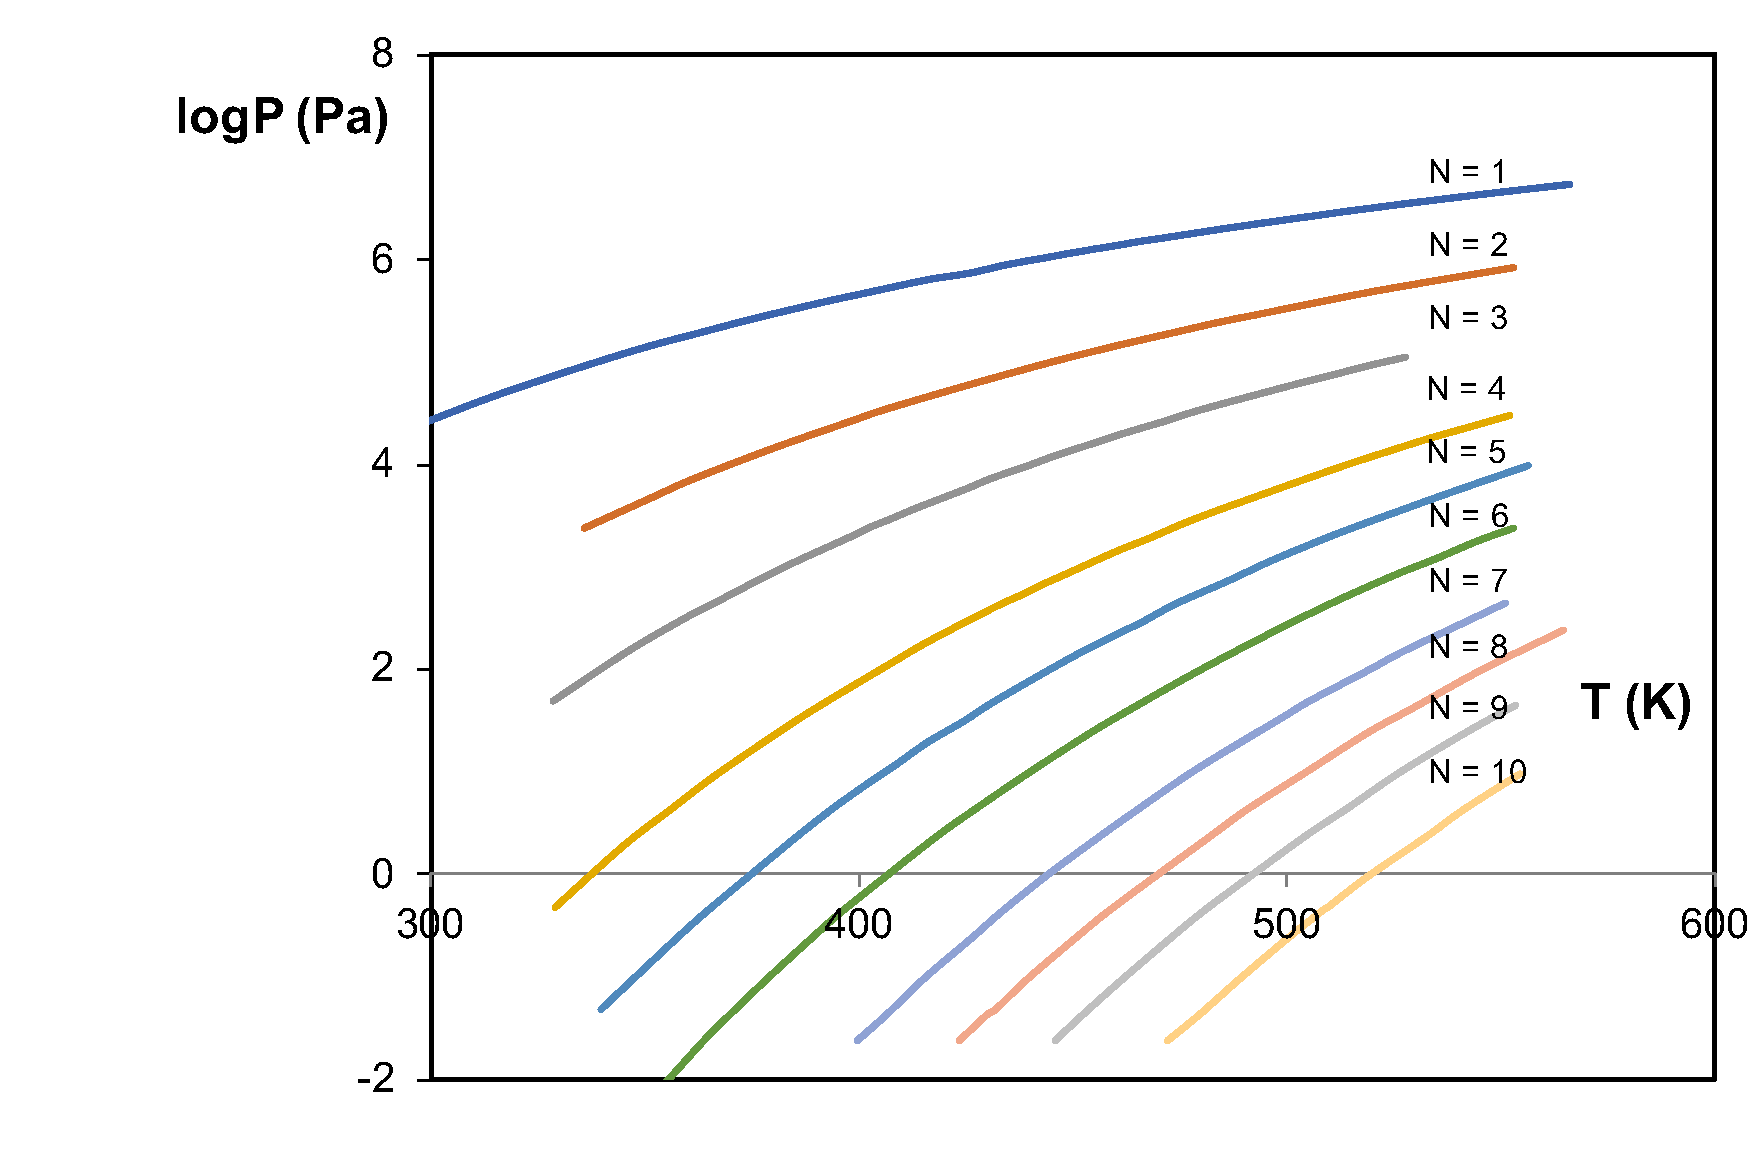
\includegraphics[width=0.6\linewidth]{PvsT}
\caption{Plot of vapour pressure vs temperature for PEO oligomers with $N$ values from 1 to 10.}
\label{fig:VPvsT}
\end{figure}

The results for vapour pressures calculated from this model are not expected to be numerically correct, but they provides a good guidance in terms of the trend of vapour pressure curves and the gaps between neighbouring $N$'s. For a specific $N$, vapour pressure increases with temperature; for a specific temperature, vapour pressure decreases with $N$. More importantly, at a given temperature, the vapour pressures of two neighbouring $N$'s have a difference of up to two orders of magnitude. However, this difference gets smaller as temperature goes higher, which indicates that it would be increasingly difficult to achieve a perfect separation, and the purification products are expected to be more polydisperse under higher evaporation temperature. In addition, the comparison between vapour pressures of PS \cite{Zhu2017a} and PEO implies that it is harder to separate individual $N$'s of PEO, because the spacings among curves are narrower for PEO than for PS, and thus the evaporation products of PEO might not be as good as PS. Evaporation temperature should never get close to 533K \cite{Choukourov2009}, which is the critical temperature where PEO begins thermal degradation in vacuum.

\section{Evaporation technique and results}

The experimental setup for evaporative purification is generally the same as the setup used for polystyrene \cite{Zhu2017a}. 96 mg of neat PEO 600 g/mol sample is placed on top of a polished silicon wafer of 2 cm $\times$ 2 cm in size and 0.3 mm in thickness. The Si wafer acts as a bottom substrate and is placed onto a Linkam hot stage in a home-built vacuum chamber. In order to collect depositing fractions, another Si wafer of 5 cm $\times$ 5 cm in size is held approximately 3 mm directly above the neat material, by thermal insulating spacers.

Before the beginning of each evaporation period, the chamber is pumped down with a dry scroll pump to an initial pressure of around 0.3 mbar. After that, we flush the chamber with nitrogen, and then evacuate it again. This process is repeated several times to flush out oxygen in the chamber, so to prevent oxidation of the polymer. Three times of flushing leads to an oxygen level of approximately $4.7 \times 10^{-6}$ times the oxygen level in atomsphere. %calculated using -29.5 inhg lower than asmosphere.
Finally, we introduce a small amount of nitrogen into the chamber, until the pressure is raised to about 170 mbar. The reason for this action is because during the evaporation, the system requires a good thermal conduction to drive away excess heat from the hot stage, so to maintain a stable temperature (with a fluctuation of less than 1K) of the material.

We start the evaporation from 393K, and the evaporated material is collected every two hours. Products from the first four hours are not collected, as they may contain impurities such as initiators. We seal the product from each period into an aluminum sample pan, in preparation for future differential scanning calorimetry measurements and mass spectroscopy measurements.

Figure \ref{fig:massvstime} shows that within each temperature region during the evaporation, the mass of material collected experiences a general decreasing trend. The mass of products collected into sample pans from the top substrates ranges from 0.2 mg to 2.9 mg. We expected that small $N$'s would come off first, and as we increased the temperature, higher $N$'s would come off later. Therefore, the neat sample would get purified through separating different $N$'s.

\begin{figure}[H]
\center
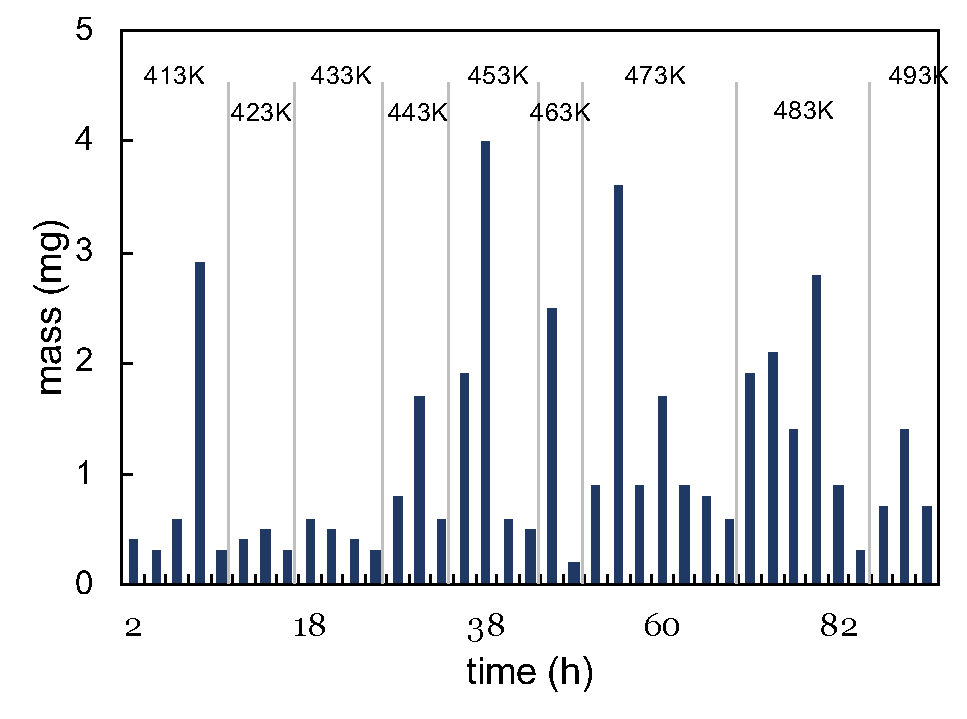
\includegraphics[width=0.5\linewidth]{massvstime}
\caption{Mass of PEO deposited on top substrate with respect to time and temperature.}
\label{fig:massvstime}
\end{figure}

\section{Results from mass spectroscopy}

To obtain information about the actual distribution of different $N$'s in each fraction, mass spectroscopy measurements were performed on several samples. Matrix Assisted Laser Desorption/Ionization – time of flight (MALDI-TOF) technique was applied, with a Bruker Autoflex Speed MALDI-TOF mass spectrometer to conduct the measurements.

A typical MALDI-TOF mass spectroscopy measurement works with the following procedure:

\begin{itemize}
\item Mix the analyte (polymer sample in our case) with appropriate matrix material (dithranol in our case).
\item Bombard the mixed material with laser. The laser energy is absorbed by the matrix, which get desorbed and ionized, and a phase transition from solid to gas takes place in the matrix material.
\item A hot plume is generated, and during the flight of both the matrix material and the analyte, collisions among particles could result in the ionization of the analyte.
\item Ions flying into the the TOF mass spectrometer are separated due to different mass ($m$)-to-charge ($z$) ratios. With the same kinetic energy, lighter ions arrive at the detector earlier than heavier ions, according to the equation:

\begin{equation}
\label{eqn_MALDI}
\dfrac{m}{z} = \dfrac{2eUt^{2}}{L^{2}}
\end{equation}

\noindent
where $e$ is the electron charge, $U$ is the voltage applied to create the electric field, $t$ is the time of flight, and $L$ is the path length.
\end{itemize}

From the spectrum generated, the exact distribution of molecular weights can be obtained, from which $M_{n}$, $M_{w}$, and PDI can be calculated.

\subsection{MALDI-TOF spectra and analysis}

MALDI measurements were carried out for 10 samples out of all the fractions, the neat PEO sample, and the leftover sample after all the evaporation periods. Figure \ref{fig:MALDIneat} is the spectrum of the neat sample, with $M_{n}$ and $M_{w}$ indicated by arrows on the plot. Figure \ref{fig:MALDIfractions} compares the purified fractions and shows the changes in molecular weight distribution during the evaporation process, with the green background spectrum being the neat sample.

\begin{figure}[H]
	\center
	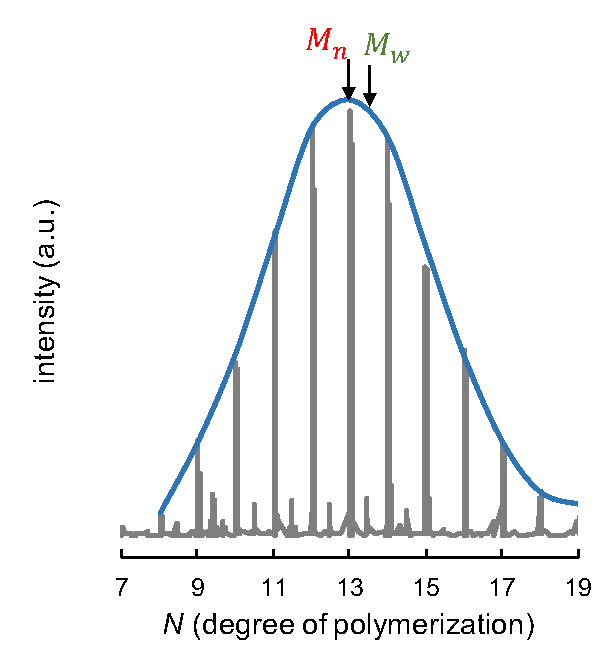
\includegraphics[width=0.4\linewidth]{MALDIneat}
	\caption{MALDI spectra of the neat sample, with $M_{n}$ and $M_{w}$ indicated.}
	\label{fig:MALDIneat}
\end{figure}

\begin{figure}[H]
\center
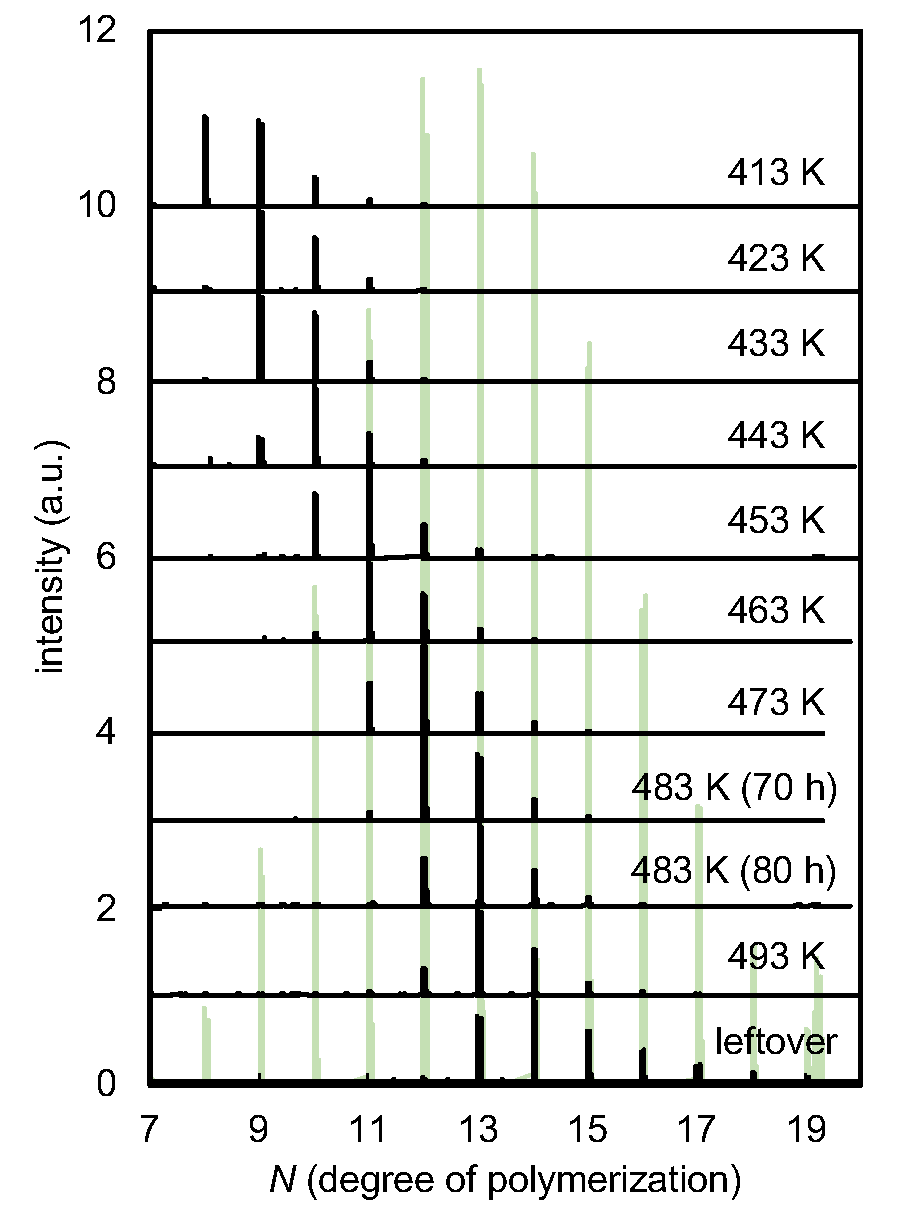
\includegraphics[width=0.4\linewidth]{MALDIfractions}
\caption{MALDI spectra of purified products (black) and neat sample (green) (80 h: 80th hour since start of evaporation).}
\label{fig:MALDIfractions}
\end{figure}

As the evaporation temperature increases, the $N$ values of the PEO chains composing each fraction shift towards higher values, ranging from 8 to 16. With the intensity of each peak, we are able to calculate their $M_{n}$, $M_{w}$, and PDI, and make quantitative comparisons. Compared to the neat sample, the $N$ composition of the products are much narrower, meaning they are highly monodisperse. The lowest PDI of the products is calculated to be 1.0052, and $(PDI - 1)$ is around six times better compared to 1.0306 of the neat sample.

\begin{figure}[H]
\center
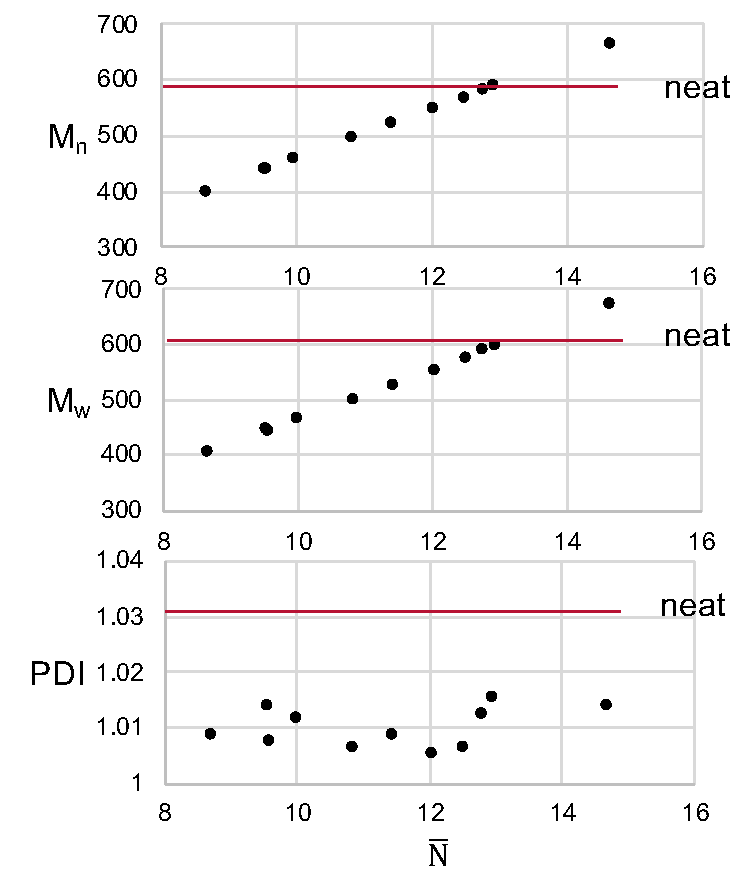
\includegraphics[width=0.4\linewidth]{fromMALDI}
\caption{$M_{n}$, $M_{w}$, and PDI comparison between products and neat sample.}
\label{fig:fromMALDI}
\end{figure}

\subsection{Evolution of $N$ during evaporation process}

So far the distribution of $N$'s at these 10 points during evaporation is obtained. However, it would be ideal if we could generate the evolution of $N$ values at any point without doing MALDI measurements on every single sample. In order to achieve this, we first plot the evolution of each $N$ value as a function of evaporation time, based on the number fraction of each $N$ in the products from different points during the evaporation process. Then we fit the ten data points for each $N$ value with Gaussian curves, which enables us to estimate the distribution of all $N$'s at any point during the evaporation (by applying interpolation only) (Figure \ref{fig:Nevolution}), and therefore calculate estimates of $M_{n}$, $M_{w}$, PDI of samples that did not have MALDI performed.

\begin{figure}[H]
  \centering
  \begin{subfigure}[b]{0.5\linewidth}
    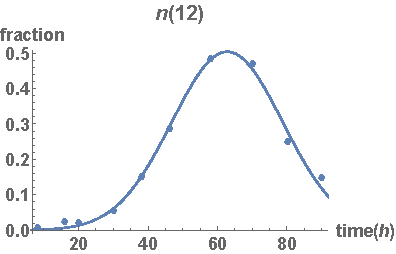
\includegraphics[width=\linewidth]{fitN12}
    \caption{Number fraction of $N$ = 12 in samples from different evaporation time.}
    \vspace{1cm}
  \end{subfigure}
  \begin{subfigure}[b]{0.5\linewidth}
    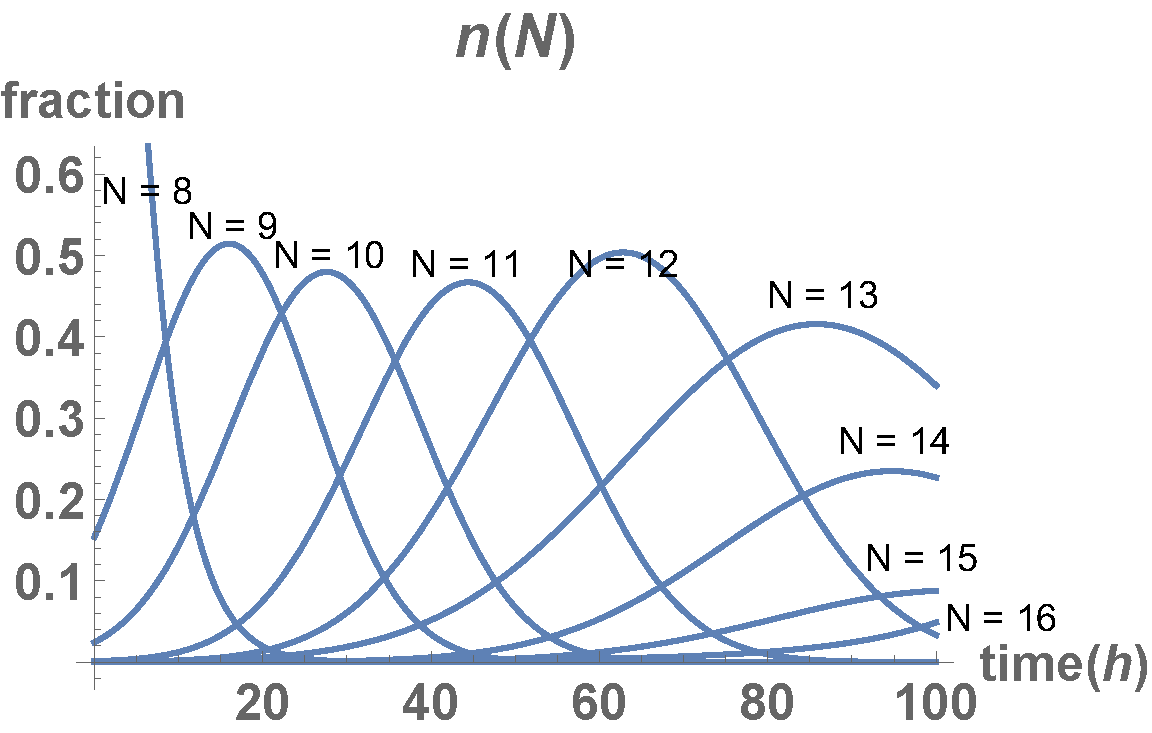
\includegraphics[width=\linewidth]{fitallNs}
    \caption{Evolution of $N$ values (from 8 to 16).}
  \end{subfigure}
  \caption{Evolution of $N$ values during evaporation process.}
  \label{fig:Nevolution}
\end{figure}

\chapter{Chain conformation analysis}\label{chap_analysis}
\graphicspath{{./analysis/graphs/}}

\section{Polymer crystallization}

\subsection{Polymer crystal models and theories}

Material systems naturally tend to stay in a lower energy state. Therefore a regular liquid upon cooling transition into solid state (the ground state), with either amorphous or crystalline state. For a polymer, the chains are entangled and aligned in all directions in liquid state, so it is much more difficult to achieve its ground state, with the monomers sitting on crystal lattice points and the chains aligned perfectly parallel with each other. However, polymers could still crystallize under proper conditions, adopting a more complex structure rather than the ideal crystalline state, and this process does not only depend on thermodynamics, but kinetics as well.

Before we look at long polymers chains, oligomers (especially linear ones) are a simpler yet close enough example in terms of crystallization. Based on X-ray crystallography results, oligomer crystals adopt a structure of stacked layers, with each layer composed of chains standing up perpendicular to the layer surface (Figure \ref{fig:oligomercrystallization}). Among neighboring layers, end-groups of the chains form the amorphous phase at the interfaces (not shown in the drawing) \cite{Strobl2007}.

\begin{figure}[H]
\center
\vspace{1 cm}
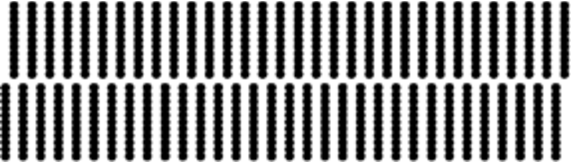
\includegraphics[width=0.5\linewidth]{oligomercrystallization}
\caption[Oligomer crystal structure.]{Oligomer crystal structure. Figure source: "The physics of polymers: Concepts for understanding their structures and behavior" by Gert Strobl, 2007 \cite{Strobl2007}.}
\label{fig:oligomercrystallization}
\end{figure}

For crystallization of polymers with higher molecular weights, however, it is impossible for the chains to completely disentangle, which requires an extremely high energy and a very long time. Limited by the nature of polymers themselves, the chains align into local crystalline domains, with some unresolved entanglements left as amorphous phases in between. Similar to oligomers, end-groups are also part of the amorphous phase. Therefore, polymer crystals are called semicrystalline crystals.

\subsubsection{Fringed micelle model}

In order to describe semicrystalline polymer crystal structures in further details, different models and theories have been proposed. One of the earliest models is fringed micelle model \cite{HerrmannKGerngrossO1930}. In this model, both the crystalline phase and the amorphous phase are present, with the crystallites existing as local domains. The micelles of crystalline parts have sizes much smaller than the chain lengths, so a single polymer chain is believed to be able to pass through several micelles, thus binding them together.

%Herrmann, K.; Gerngross, O.; Abitz, W. Zur rontgenographischen Strukturforschung des gelatinemicells. Z. Phys. Chem. B 1930, 10, 371–394.

\begin{figure}[H]
\center
\vspace{1 cm}
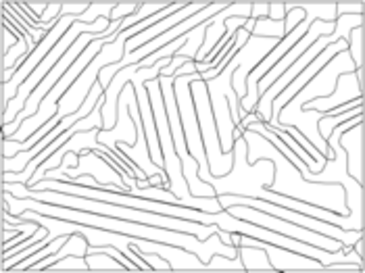
\includegraphics[width=0.3\linewidth]{fringedmicelle}
\caption[Fringed micelle model of polymer crystal structure.]{Fringed micelle model of polymer crystal structure. Figure source: "Principles of polymer chemistry" by Paul J. Flory, \textit{Cornell University Press}, 1953 \cite{Flory1953}.}
\label{fig:fringedmicelle}
\end{figure}

However, there were some problems with fringed micelle model. According to the calculation of free energy, it was found that there would be a large conformational entropy loss for the amorphous chains if this model was true \cite{Flory1962}. In addition, experimentalists observed evidences of large crystallites - "sperulites", which have a strong preference in terms of the alignment of chains, and are highly symmetrical instead of a random distribution of crystallites \cite{Geil1964}. Together with some other flaws and contradictions found with the model itself \cite{Zachmann1967,Zachmann1969}, people began to doubt fringed micelle model and try to find other ways to describe semicrystalline polymer crystals.

\subsubsection{Folded chain model} \label{sec: folded chain model}

As the fringed micelle model was being questioned, some crucial experimetal observations led to the birth of a new model of polymer crystals---the folded chain model. The concept of chain-folding was actually first proposed by Storks \cite{Storks1938}. He observed unstretched films of gutta-percha through electron diffraction measurements, and found that the films are composed of large crystallites with the chain axis perpendicular to the film surfaces. The thickness of the films are much smaller than the chain lengths, which led to Storks' proposal that the chains need to fold themselves inside the film.  At that time, fringed micelle model was still dominating the directions of polymer crystallization researches, so his results and proposal did not receive much attention. Later, several researchers \cite{JACCODINE1955,Till1957,Keller1957} studied polymer single crystals and found that they have smooth surfaces, with heights of about 10 nm, which is also much smaller than the chain lengths. The chains are believed to fold themselves back and forth in each lamella, and when the polymer solution concentration is high enough, or when the polymer crystallizes from a melt, mutiple lamellae stack together to form a crystal. These observations helped the development of folded chain model, which from then on became the most widely accepted model of polymer crystals. 

Now it is clear that the chains fold in crystal, and next step would be to determine the way of chain folding. After the chain gets to the amorphous interface and fold itself back, it is not clear where it re-enters the lamella. There have been a large number of studies on this \cite{Kovacs1975,Yoon1979,Keller1979} and two major models have been proposed: adjacent re-entry model and random re-entry model.

As adjacent re-entry model describes, after a chain escapes the lamella and makes a fold, it turns right back and inserts into the neighboring site. In this way, the lamellae created have relatively smooth surfaces, as Figure \ref{fig:adjacent} shows.

\begin{figure}[H]
\center
\vspace{1 cm}
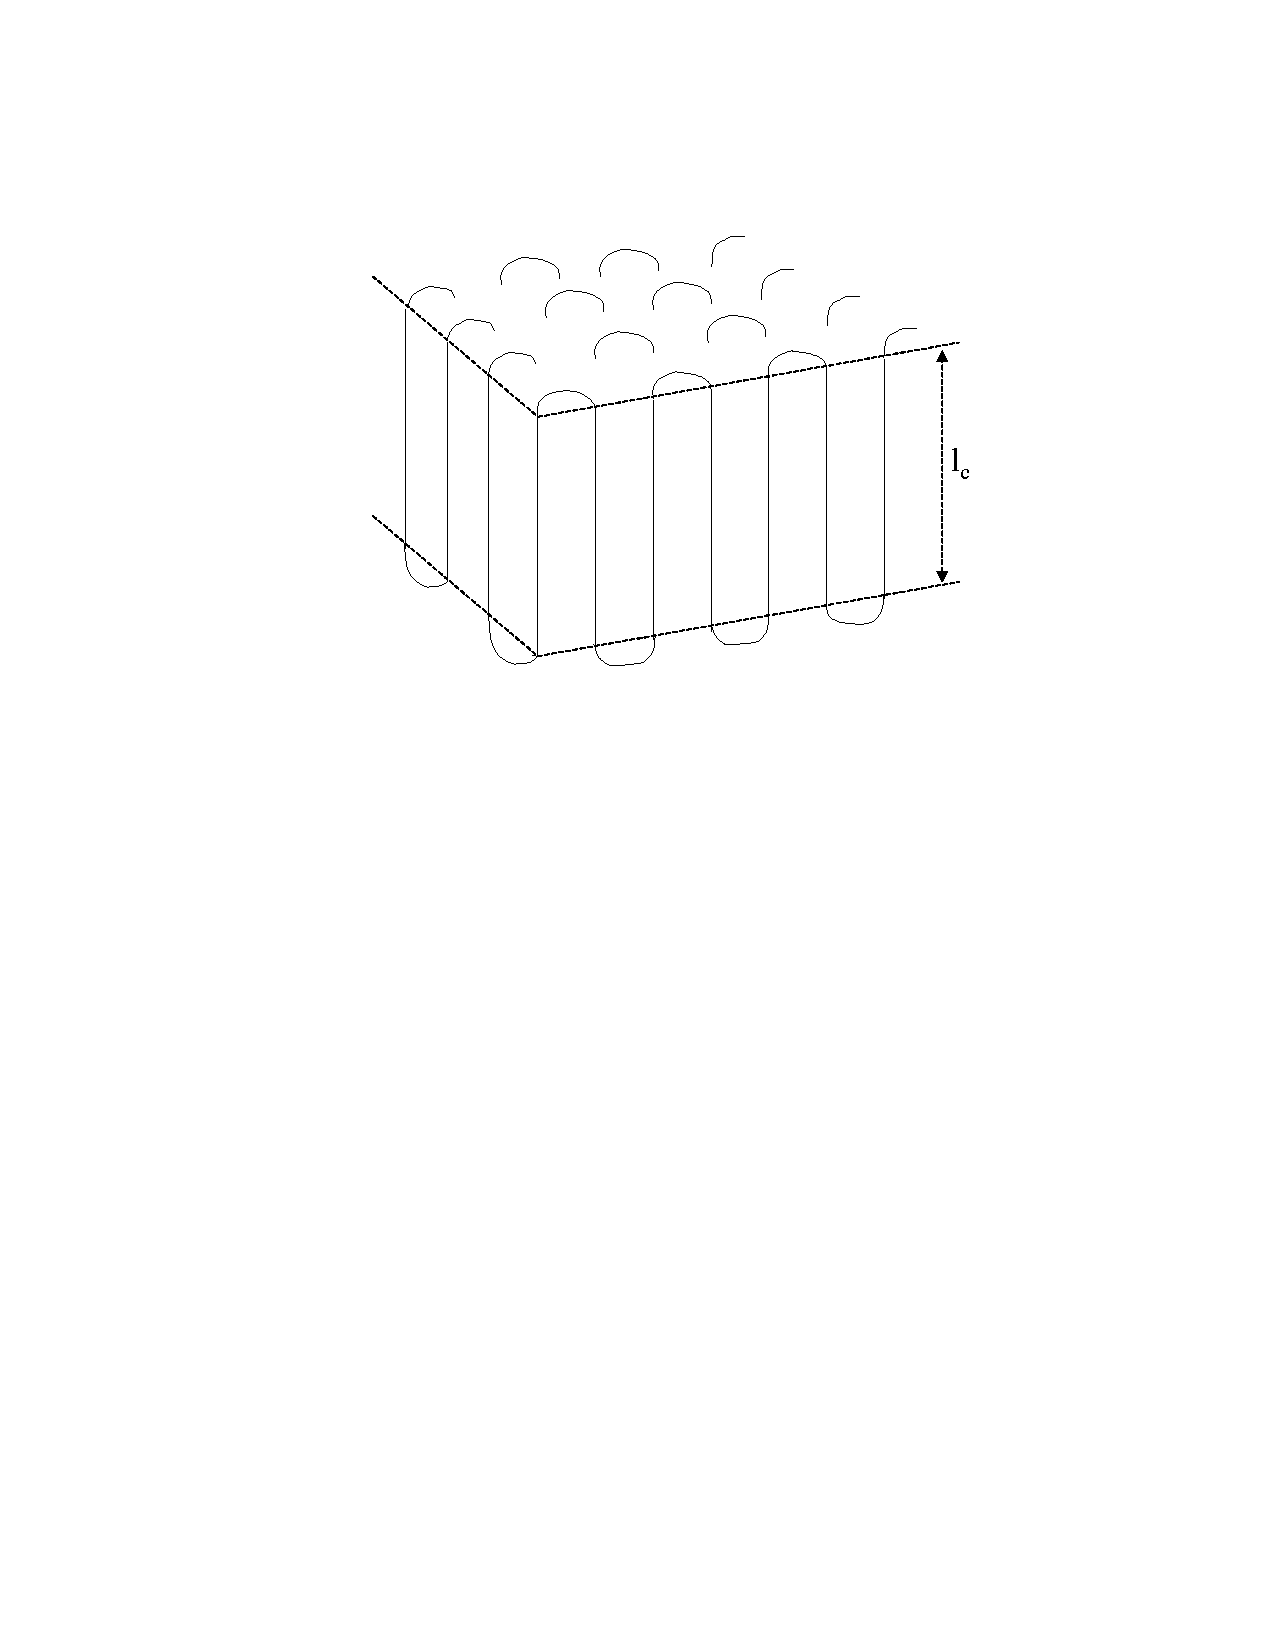
\includegraphics[width=0.4\linewidth]{adjacent}
\caption[Adjacent re-entry model of polymer crystals.]{Adjacent re-entry model of polymer crystals. Figure source: "Advanced High and Strength Steels. Chapter 2. Literature Review", pages 7–78 \cite{High}.}
\label{fig:adjacent}
\end{figure}

Random re-entry model is also known as switchboard model. Instead of folding right back into the neighboring site on the same lamella, a chain that emanated from the lamellar surface could either float on the interface and walk into a further site, or even enters a neighboring lamella, which leads to a completely random arrangement on the interfaces of lamellae and amorphous regions (Figure \ref{fig:random}).

\begin{figure}[H]
\center
\vspace{1 cm}
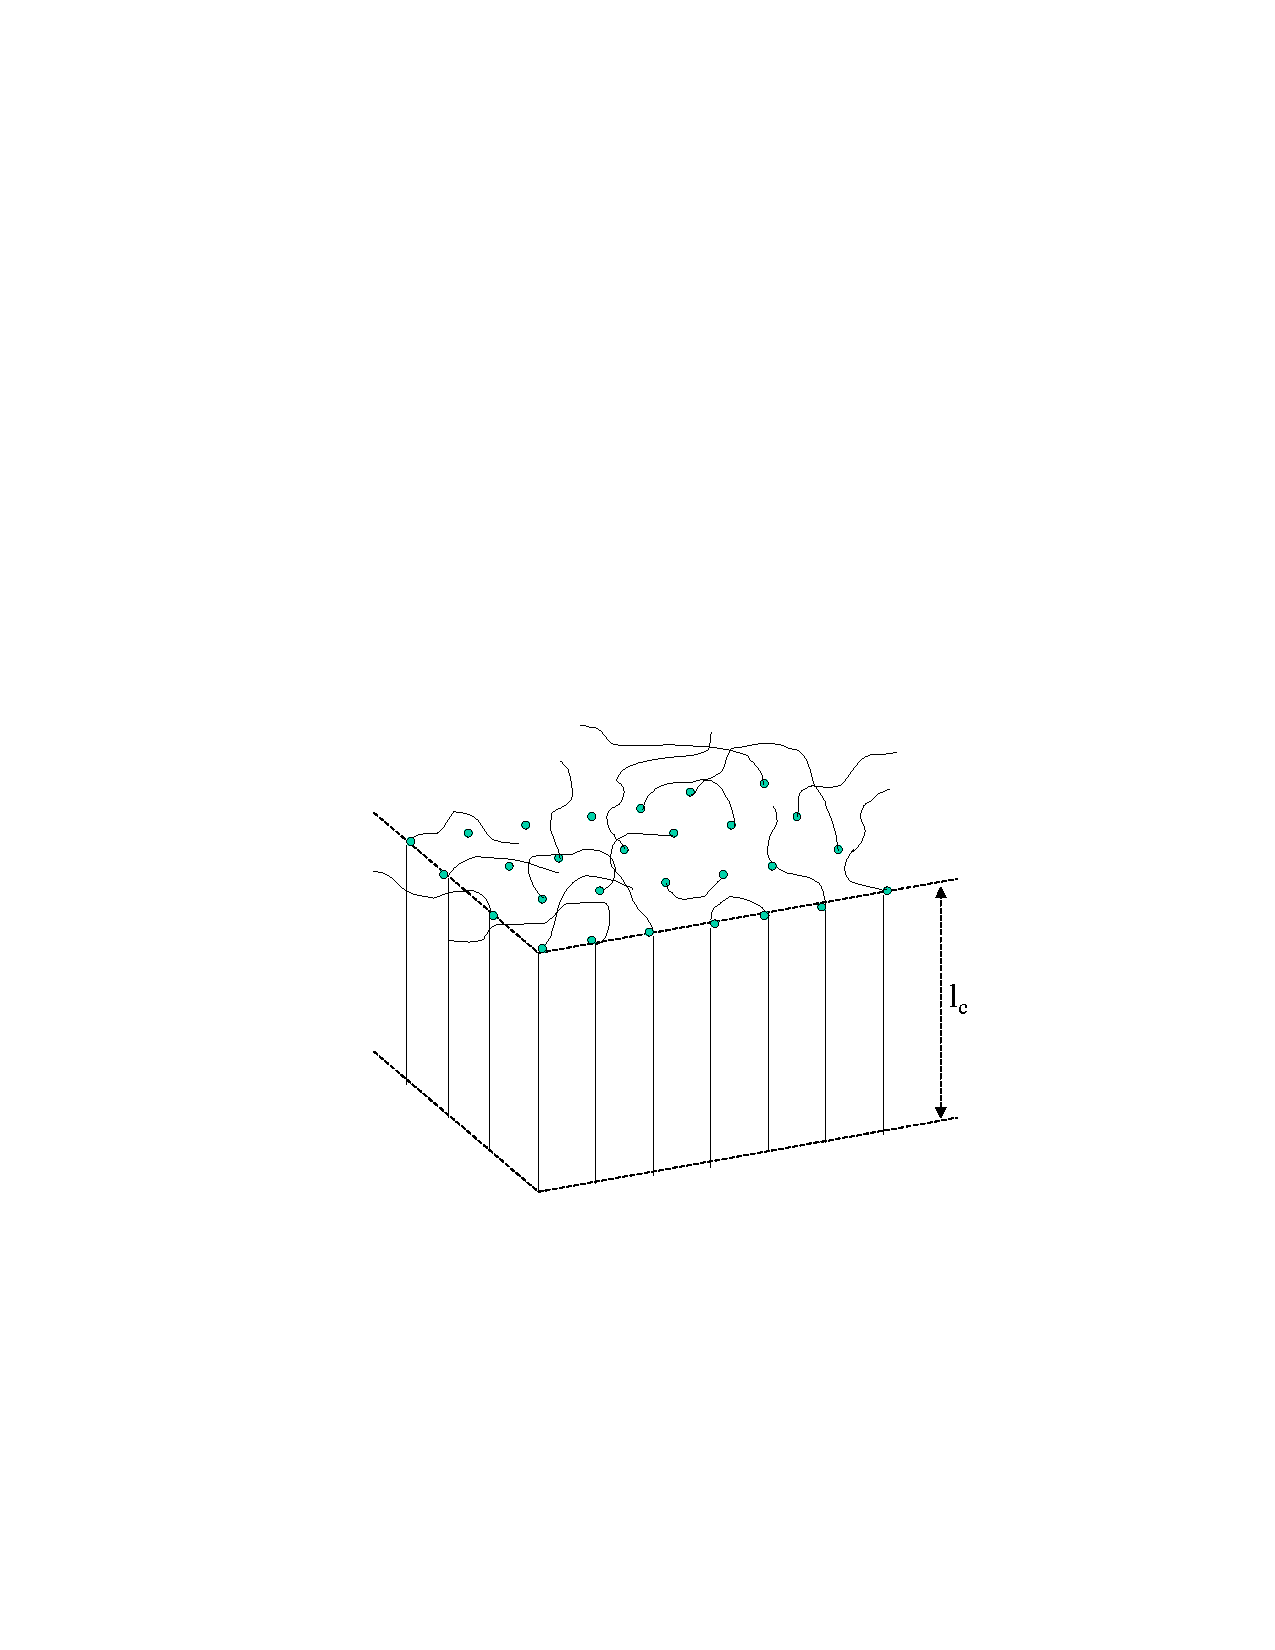
\includegraphics[width=0.4\linewidth]{random}
\caption[Random re-entry model of polymer crystals.]{Random re-entry model of polymer crystals. Figure source: "Advanced High and Strength Steels. Chapter 2. Literature Review", pages 7–78 \cite{High}.}
\label{fig:random}
\end{figure}

Adjacent re-entry model would result in a much more thermodynamically favorable conformation with a lower entropy. However, in a real situation of polymer crystallization, twisting, misalignment, and entanglements of the long chains prevent them from relaxing and aligning perfectly in regular folds. Instead, regions consisting too many entanglements are more likely to be shifted to the surfaces and contribute to the amorphous phase \cite{Strobl2007}. Taking both thermodynamics and kinetics factors into account, real polymer crystal lamellae are normally composed of both adjacent re-entries and random re-entries. It should be noted that in real cases, chain-folding also depends on more factors: chain lengths, flexibility of chains, crystallization temperature, cooling rate, chain defects, etc.
 
\subsection{Thermodynamics of polymer crystallization} \label{Thermodynamics of polymer crystallization}

Thermodynamics is the fundamental rule that polymer chains obey during crystallization. The most favorable state for polymers is that with the lowest possible free energy $G$. $G$ is lower for melt than for crystals at high temperatures, while it is lower for crystals than for melt at low temperatures. The equilibrium melting point $T_{m}^{\infty}$ is defined as the temperature at which the liquid state and the solid state have the same free energy. Therefore, the change in Gibbs free energy, $\Delta G$, is equal to zero during melting or crystallization transition at thermodynamic equilibrium:

\begin{equation}
\label{eqn_deltaG}
\Delta G = \Delta H - T_{m}^{\infty} \Delta S = 0
\end{equation}

\begin{equation}
\label{eqn_Tminfinity}
T_{m}^{\infty} = \dfrac{\Delta H}{\Delta S}
\end{equation}

In practical cases, the crystallization temperature $T_{c}$ is always lower than the melting temperature $T_{m}$, and their difference is defined as the supercooling $\Delta T$. This is mainly due to the nucleation and growth mechanism during crystallization. A nucleus must be present to initialize the growth of a crystal, and when there is no present nuclei, the temperature needs to keep decreasing until the melt itself starts a primary nucleation. This mechanism will also be further discussed in Chapter \ref{chap_growth}. Compared to regular crystals, $\Delta T$ of polymers could be as large as 20 to 30 K, resulting from the metastable chain-folding nature of polymers \cite{Hu2013}.

Equation \ref{eqn_Tminfinity} tells us that the equilibrium melting temperature depends on both enthalpy and entropy of the system. However, the effect of surface energy and crystal size has not been considered. For a real polymer crystal, shape and size of the lamella would directly affect its melting point, and this effect could be examined through thermodynamics.

Let us start with an infinitely large crystal, and from conventional thermodynamic viewpoints it is considered not to involve surface energy. Therefore its melting point is believed to be $T_{m}^{\infty}$.

\begin{figure}[H]
	\center
	\vspace{1 cm}
	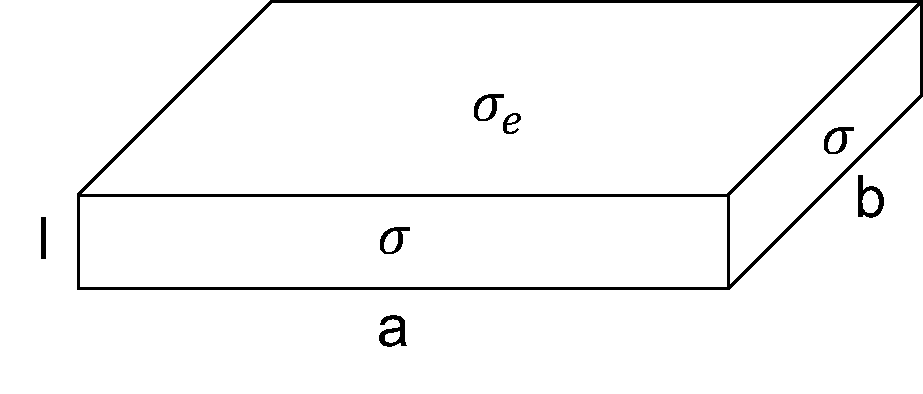
\includegraphics[width=0.5\linewidth]{lamella}
	\caption{Schematic drawing of a polymer crystal lamella.}
	\label{fig:lamella}
\end{figure}

Now assume a lamella (Figure \ref{fig:lamella}) with length $a$, width $b$, and height $l$, where $a \gg l$, and $b \gg l$. The surface energy per unit area of the top and bottom surfaces is $\sigma_{e}$, and the surface energy per unit area of the side surfaces is $\sigma$. This lamella with the finite size effect could be considered as a quasi-two dimensional object with one-dimensional confinement \cite{Zhang2016}. The free energy per unit mass on melting is $\Delta g$, and the total free energy $\Delta G$ on melting consists of the energy required to create new surfaces and the energy of fusion for the bulk:

\begin{equation}
\label{eqn_delta G lamella}
\Delta G = 2(a+b)l\sigma + 2ab\sigma_{e} - abl\Delta g
\end{equation}

\noindent
and with $\sigma_{e}\gg\sigma$, $a\gg l$, $b\gg l$, the total free energy is then:

\begin{equation}
\label{eqn_delta G lamella reduced}
\Delta G = 2ab\sigma_{e} - abl\Delta g
\end{equation}

At melting temperature $T_{m}$, $\Delta G = 0$, which leads to:

\begin{equation}
\label{eqn_delta g lamella}
\Delta g (T_{m}) = \dfrac{2\sigma_{e}}{l}
\end{equation}

Once again, for an infinitely large crystal, we have:

\begin{equation}
\label{eqn_delta g large}
\Delta g (T_{m}^{\infty}) = \Delta h (T_{m}^{\infty}) - T_{m}^{\infty}\Delta s (T_{m}^{\infty}) = 0
\end{equation}

Assuming between $T_{m}$ and $T_{m}^{\infty}$, the enthalpy and entropy could be treated as invariant, we further have:

\begin{equation}
\label{eqn_delta g}
\Delta g (T_{m}) = \Delta h (T_{m}) - T_{m}\Delta s (T_{m})
\end{equation}

Combining Equation \ref{eqn_delta g large} and Equation \ref{eqn_delta g}, we are able to generate:

\begin{equation}
\label{eqn_delta g 2}
\Delta g (T_{m}) = \Delta h (T_{m}) - T_{m}\dfrac{\Delta h (T_{m})}{T_{m}^{\infty}}
\end{equation}

Now with Equation \ref{eqn_delta g lamella} and Equation \ref{eqn_delta g 2}, we finally obtain the relation between the thickness of a lamella and its melting temperature:

\begin{equation}
\label{eqn_GT}
T_{m} = T_{m}^{\infty} (1 - \dfrac{2\sigma_{e}}{l \Delta h})
\end{equation}

\noindent
which is the well-known Gibbs Thomson equation. It has been applied to many polymers with linear structure and has proved to provide reliable predictions of the melting temperature as a function of lamella thickness \cite{KojiYamada2003}. With a larger thickness, the finite size effect is weaker, and the melting temperature $T_{m}$ of the lamella would be closer to the equilibrium melting temperature $T_{m}^{\infty}$.

\section{PEO crystallization}

In terms of crystallization, PEO is one of the most intensively studied polymers, together with Poly(Ethylene) and n-alkanes. With a linear structure, these polymers all crystallize very easily. As a semicrystalline polymer, PEO chains fold into lamellar structures during crystallization process, and multiple lamellae stack up to form the whole crystal \cite{Arlif1966}. In our case, we focus on low molecular weight PEO, so crystallization should be even easier since the chains are relatively short and thus need fewer times of folding. When the number of folds changes, the thickness of the lamella varies, which has a direct influence on the melting temperature of the crystal lamella.

\subsection{Crystal structure}

PEO crystals have monoclinic unit cells, with the chains adopting a structure of 7/2 helix with trans-gauche-trans conformation. In this conformation, seven monomeric units form two periods of the helix, which is 1.93 nm long \cite{Yoshihara1964}. As shown in Figure \ref{fig:PEOhelix}, every bond is rotated by a certain angle with respect to the c-axis (vertical axis) of the lamella, and the projection length of one monomer on the c-axis, $l_{c}$, is 0.278 nm \cite{Takahashi1973}.

\begin{figure}[H]
\center
\vspace{1 cm}
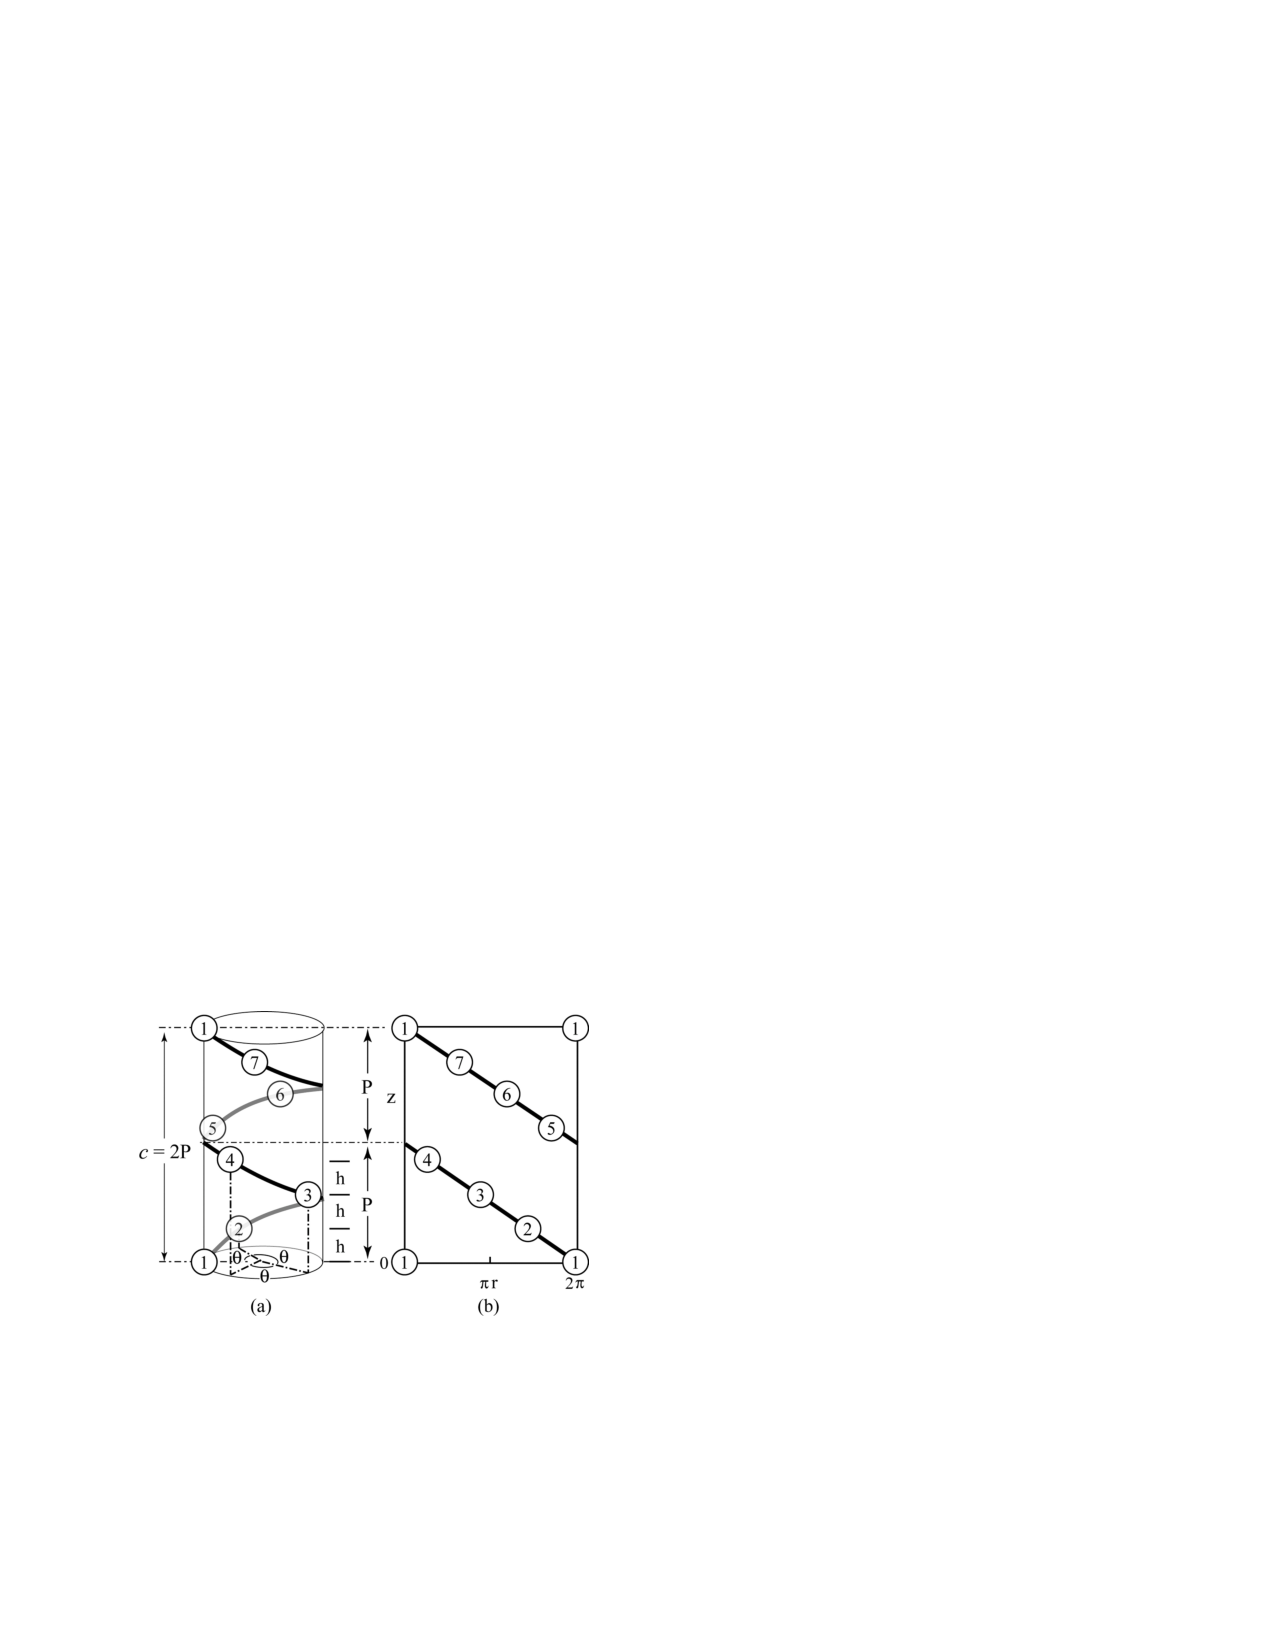
\includegraphics[width=0.7\linewidth]{helix}
\caption[7/2 helix structure (a) and its radial projection (b).]{7/2 helix structure (a) and its radial projection (b). Circles with numbers represent monomers. Pitch length, P, and unit length, h, represent the axial lengths of one helical turn and one monomer, respectively. $\theta$ represents the angle between two monomers around the helical axis, and $r$ represents the helix radius. Figure source: "Revisiting the Molecular Structure of Collagen" by Kenji Okuyama, \textit{Connect. Tissue Res.}, 49(5):299-310, 2008 \cite{Okuyama2008}.}
\label{fig:PEOhelix}
\end{figure}

Low molecular weight PEO fractions, or PEO oligomers, crystallize with chains folded a small number of times, or even fully extended \cite{Kovacs1975,Kovacs1977}. The number of folds depends on many factors including crystallization temperature, chain length, cooling rate, etc. The thickness of the lamella $L$ is thus determined by the number of folds $n$ and the chain length $\lambda$:

\begin{equation}
\label{eqn_thickness}
L = \dfrac{\lambda}{1+n} = \dfrac{N l_{c}}{1+n}
\end{equation}

\noindent
where $N$ is the number of monomers in a chain, or the degree of polymerization. Especially for fully extended chains, $n = 0$, and the thickness of the lamella is equal to the chain length.

In terms of chain folding, we have also discussed about the two different chain re-entry models in \ref{folded chain model}: adjacent re-entry model and random re-entry model. In the case of PEO oligomers, the chains are relatively short, and there are not as many entanglements among the chains, so we could expect more adjacent re-entries in the lamellae.

\subsection{Melting points of PEO oligomers} \label{Tm and Yeates}

Gibbs Thomson equation (Equation \ref{eqn_GT}), enables one to build the relation between melting points and other physical parameters of a polymer crystal. In order to be consistent with other researches on PEO melting transitions, here we make some modifications to the original equation:

\begin{equation}
\label{eqn_GT2}
T_{m} = T_{m}^{\infty} (1 - \dfrac{2SV}{L \Delta H})
\end{equation}

\noindent
where $S$ is the surface free energy of the interface between the crystalline and the amorphous phase, and $V$ is the molar volume of a crystallizable repeat unit \cite{Pfefferkorn2011}. In this equation, $T_{m}^{\infty}$, $V$, and $\Delta H$ are constants that have been determined for PEO.

Melting transitions of PEO have been intensively studied through various experimental methods and from different theoretical aspects. One of the fundamental researches is of our particular interest and is worth being reviewed. Relatively monodisperse PEO oligomers with the degree of polymerization ranging from 9 to 45 were produced through step-wise syntheses by Yeates \textit{et al} \cite{Yeates1984}. Melting points of these fractions were measured, and compared to those of commercially available samples, which are much more polydisperse. Their results are shown in Figure \ref{fig:Yeates}.

\begin{figure}[H]
\center
\vspace{1 cm}
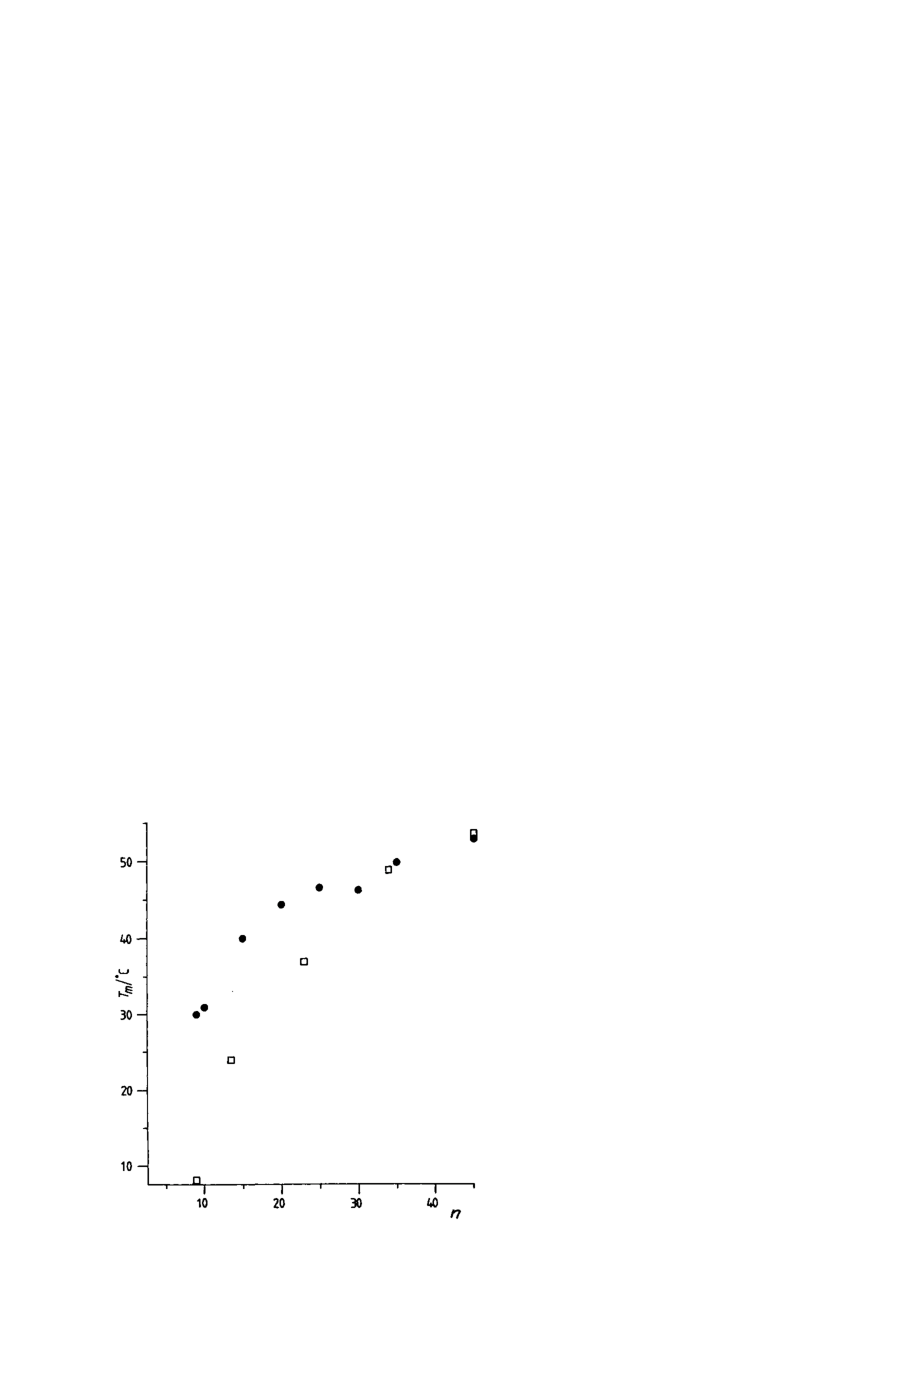
\includegraphics[width=0.5\linewidth]{Yeates}
\caption[Melting points vs degree of polymerization for monodisperse (black dots) and polydisperse (empty boxes) PEO oligomer samples.]{Melting points vs degree of polymerization for monodisperse (black dots) and polydisperse (empty boxes) PEO oligomer samples. Figure source: "Ethylene glycol oligomers" by Stephen G. Yeates \textit{et al}, \textit{Makromol. Chemie}, 185(8):1559-1563, aug 1984 \cite{Yeates1984}.}
\label{fig:Yeates}
\end{figure}

Melting points of monodisperse samples are notably higher than those of polydisperse samples in general, and the difference is especially large for small N values. This observation indicates that polydispersity has a big influence on melting temperature, and in fact became the motivation that we conducted crystallization experiments with our purified samples, so that we could further investigate this phenomenon.

As a matter of fact, this observation has attracted much attention from researchers. One of explanations that have been proposed suggests that the $T_{m}$ difference could be related to the chain end-groups \cite{Percec1989}. In a relatively monodisperse sample, chains have roughly the same length, which makes it easier to create a smooth lamellar surface, and the end-groups would be incorporated in the crystalline array. However, in a polydisperse sample, the distribution of chains results in a more disordered lamellar surface, so some of the end-groups have to be incorporated in the amorphous phase. Because of the difference in the incorporation of chains ends, polydisperse crystals would have lower crystallinity and higher entropy, which leads to a higher melting temperature.

\section{Basics of differential scanning calorimetry}

\subsection{Phase transitions in polymers}

Phase transitions are a major aspect to study in a polymer's properties. In regular materials, phase transitions normally refer to the transitions between solid, liquid, and gaseous states. For polymer materials, we focus more on the transition between solid state and liquid state, i.e., melting transition and crystallization transition, which occur in the crystalline regions in polymers. In addition, there is a unique transition that takes place in the amorphous regions in polymers -- glass transition.

In crystalline regions, materials stay in the form of disordered melt at temperatures above $T_{m}$, and ordered crystalline solid below $T_{m}$. At melting temperature $T_{m}$, the material experiences a discontinuity in the specific volume, and absorbs or releases a certain amount of heat (depending on the direction of transition), which is called latent heat. Such transitions are classified as first-order phase transitions \cite{Jaeger1998}. 

\begin{figure}[H]
	\center
	\vspace{1 cm}
	\begin{tikzpicture}[domain=0:4] 
	\begin{axis}[
	ticks=none,
	axis x line=middle,axis y line=left,
	xlabel = {$T$},
	ylabel = {$V$},
	xmin=0,xmax=9,
	ymin=0,ymax=9,ylabel style={rotate=-90},
	]
	\addplot [mark=none] coordinates {(1,1) (5,2)};
	\addplot [mark=none, dashed] coordinates {(5,2) (5,5)};
	\addplot [mark=none] coordinates {(5,5) (8,8)};
	\addplot [mark=none, red] coordinates {(5,0) (5,2)};
	\addplot [mark=none] coordinates {(5.5,0)} node[above]{$T_{m}$};
	\addplot [mark=none] coordinates {(3,1.5)} node[above]{crystal};
	\addplot [mark=none] coordinates {(6,6.5)} node[above]{liquid};
	\end{axis}
	\end{tikzpicture}
	\caption{Temperature of specific volume of a polymer under melting or crystallization transition, where $T$ is the temperature and $V$ is the specific volume.}
	\label{fig:V vs T for Tm}
\end{figure}

In amorphous regions, materials stay in the form of disordered liquid (viscous or rubbery) at temperatures above $T_{g}$, and transform into disordered solid below $T_{g}$ \cite{InternationalOrganizationforStandardization2013}. At glass transition temperature $T_{g}$, specific volume of the material evolves continuously, and there is no latent heat involved. Such transitions are classified as second-order phase transitions \cite{Jaeger1998}. Although there is no latent heat, heat capacity of the sample does change, as indicated by the slope change in Figure \ref{fig:V vs T for Tg}. One thing to note is that glass transition normally occurs in a range of temperatures, rather than at a single point, and it always occur below $T_{m}$. This is because glass state is not a thermodynamically-stable state, and the measurement result of $T_{g}$ depends on factors such as the polymer's thermal history and the heating or cooling rate.

\begin{figure}[H]
	\center
	\vspace{1 cm}
\begin{tikzpicture}[domain=0:4] 
\begin{axis}[
ticks=none,
axis x line=middle,axis y line=left,
xlabel = {$T$},
ylabel = {$V$},
xmin=0,xmax=9,
ymin=0,ymax=9,ylabel style={rotate=-90},
]
\addplot [mark=none] coordinates {(1,2) (5,4)};
\addplot [mark=none] coordinates {(5,4) (8,8)};
\addplot [mark=none, red] coordinates {(5,0) (5,4)};
\addplot [mark=none] coordinates {(5.5,0)} node[above]{$T_{g}$};
\addplot [mark=none] coordinates {(3,3)} node[above]{glass};
\addplot [mark=none] coordinates {(6,6)} node[above]{liquid};
\end{axis}
\end{tikzpicture}
	\caption{Temperature of specific volume of a polymer under glass transition, where $T$ is the temperature and $V$ is the specific volume.}
	\label{fig:V vs T for Tg}
\end{figure}

One major difference between first-order and second-order phase transitions is their driving force. In a melting transition, the process is driven by thermodynamics, as the crystalline state is the thermodynamic ground state at low temperatures. However, the glass state is not a ground state, with the chains not being fully ordered. It has been suggested in some theoretical predictions that given long enough relaxation time, the glass state finally transform into crystalline state \cite{Gotze2009}. Instead of being thermodynamically driven, glass transition is normally considered as a kinetic transition.

\subsection{Working mechanism of differential scanning calorimetry}

The products pressed into Al pans previously are characterized with a differential scanning calorimeter (DSC) (Q100, TA Instruments). DSC is an instrument that measures the change of heat flow to the sample material within a controlled temperature range. Inside a typical DSC there are two metal (Al commonly) pans, with one acting as the sample pan and another empty pan acting as a reference. Through precise heating and cooling control with a feedback mechanism, the two pans are maintained at the same temperature at any time during the scanning measurement. At temperatures where phase transitions of the sample material takes place, the heat capacity of the sample changes, which requires the computer to adjust the amount of heat flow provided, in order to always keep the two pans at the same temperature. Heat flow $\dfrac{dQ}{dt}$ could be obtained as a function of temperature, which depends both on the heat capacity $C_{p}$ of the sample and the scanning rate $q$:
\begin{equation}
\label{eqn_DSC}
\dfrac{dQ}{dt} = \dfrac{dQ}{dT}\cdot\dfrac{dT}{dt} = C_{p} q
\end{equation}

By plotting the difference in heat flow to the two pans with respect to temperature, thermal transitions the sample material experienced during the set range of temperature, such as crystallization, melting, and glass transition, could be determined. Figure \ref{fig:DSCcurveeg} is a typical DSC curve. When the scanning rate is constant, first-order transitions appear as peaks on the DSC curve. Crystallization appears as an exothermic peak on the cooling curve, and melting appears as an endothermic peak on the heating curve. The difference observed between the crystallization temperature $T_{c}$ and the melting temperature $T_{c}$ is supercooling $\Delta T$. Note that here in this figure crystallization and melting are presented on the same curve for the sake of neatness, but they in fact occur on separare curves.

\begin{figure}[H]
\center
\vspace{1 cm}
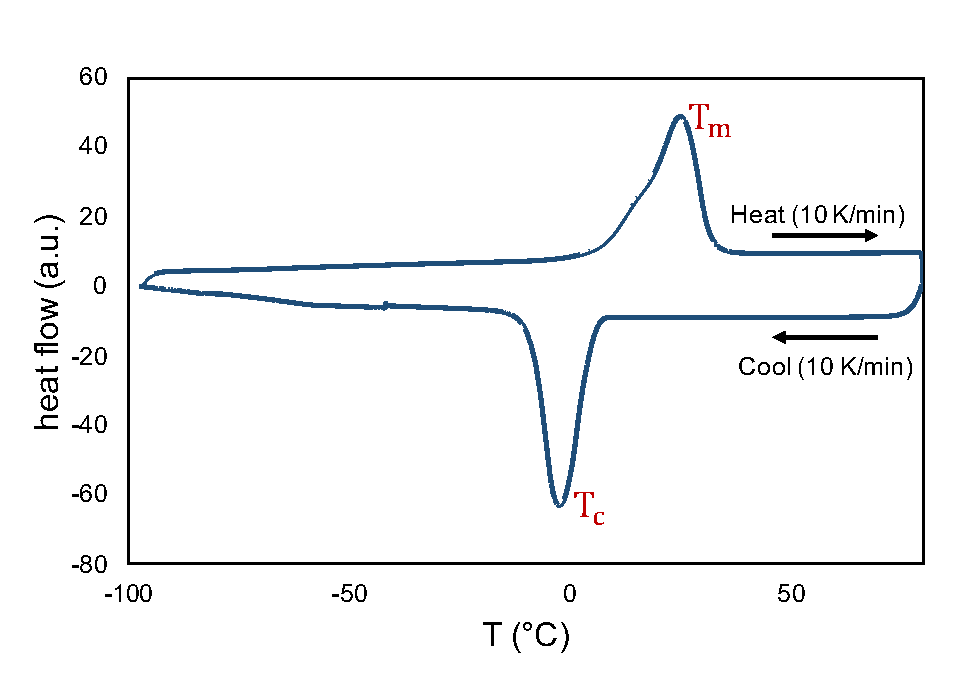
\includegraphics[width=0.6\linewidth]{DSCcurveeg}
\caption[A typical DSC curve for a polymer sample.]{A typical DSC curve for a polymer sample. Figure source: "Thermoanalytical Methods in Verifying the Quality of Biodiesel" by Marcelo Y Misutsu \textit{et al}, \textit{Biofuels - Status Perspect.}, 2015 \cite{Misutsu2015}.}
\label{fig:DSCcurveeg}
\end{figure}

\section{Results from differential scanning calorimetry}

The following running process is performed on each product: equilibrate at 353 K (to fully melt all crystal); isothermal for 5 min; ramp 10 K/min to 173 K (to crystallize the sample); isothermal for 5 min; ramp 10 K/min to 353 K; isothermal for 5 min; ramp 10 K/min to 173 K; isothermal for 5 min; ramp 10 K/min to 353 K. With two runs of the same procedure, we examine the reproducibility of the results.

\subsection{Melting temperature}

From the DSC curves of each fraction, we determined their melting temperature, $T_{m}$, as shown in Figure \ref{fig:Tm}. Most of the samples show a double-peak pattern, with a lower $T_{m1}$ and a higher $T_{m2}$. Each measurement is carried out for more than once, and the $T_{m}$ values from separate measurements normally vary within $\pm$ 2 degrees. $\bar{N}$ is the average $N$ value of each sample, which is interpolated linearly based on the 10 samples measured with MALDI. In general, the melting temperatures behave as Gibbs Thomson relation describes, with the higher $N$ values (longer chains) showing higher melting temperatures.

\begin{figure}[H]
\center
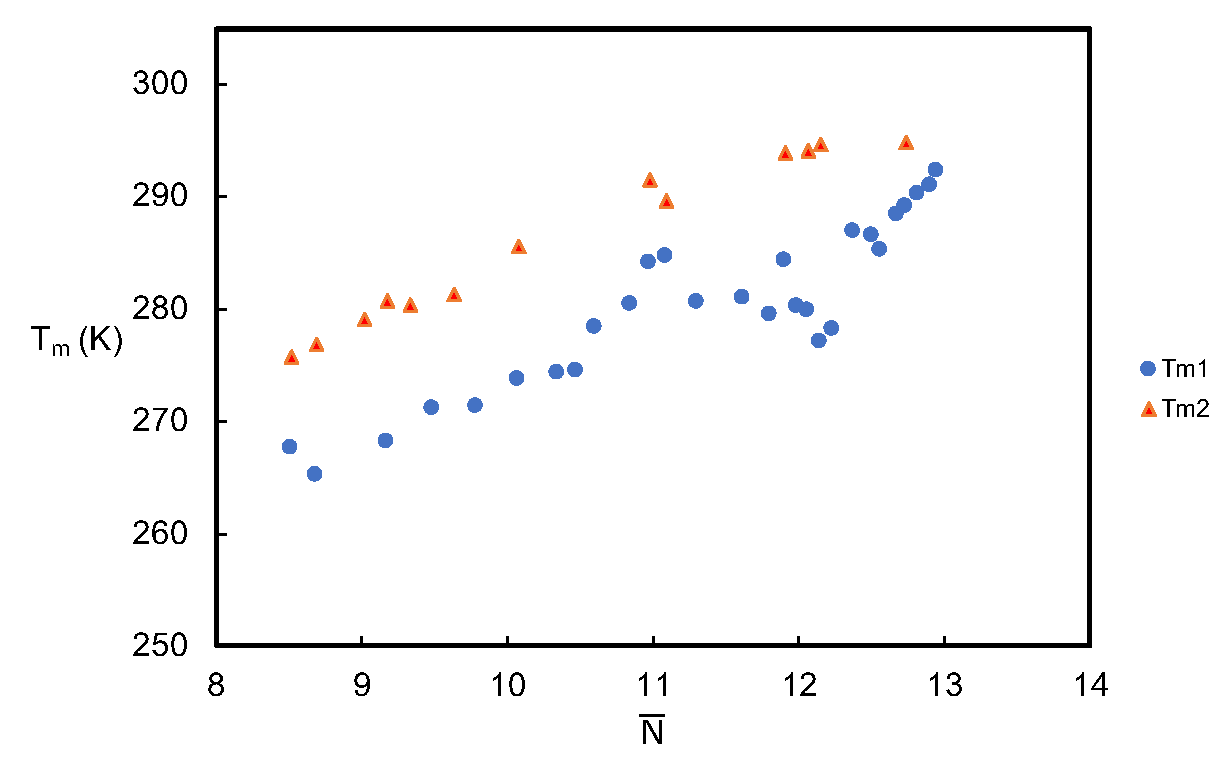
\includegraphics[width=\linewidth]{Tm}
\caption{Melting temperature of purified fractions.}
\label{fig:Tm}
\end{figure}

\subsubsection{Chain-folding analysis based on $T_{m}$}

In figure \ref{fig:Tm}, it is obviously seen that the data points potentially lie on two parallel curves, which brings our assumption that they could correspond to two types of chain-folding modes in the crystal lamellae, with the higher $T_{m}$'s being extended chains (larger thickness), and the lower $T_{m}$'s being once-folded chains (smaller thickness).

In order to validate our assumption, we apply Equation \ref{eqn_GT} to see if we are able to get a good fit with the two series of data. Parameters for PEO present in this equation, including $T_{m}^{\infty}$ \cite{Buckley1975}, $V$ \cite{Wong2015}, $\Delta H$ \cite{Yave2010} are found in the literature. Interfacial tension $S$ is dependent on the mode of chain-folding, as both chain ends and chain folds contribute to the amorphous phase, and they lead to different interfacial tensions with respect to the crystalline phase.

Interfacial tension of chain folds, $S_{folds}$, could be obtained from parameters of PEO chains with large enough molecular weights. This is because in the crystal lamellae of long chains, the number of chain folds are much greater than that of chain ends, and thus $S$ is dominated by chain folds. For long PEO chains, crystal lamellar thickness $L$ is normally on the order of 10 nm \cite{Okerberg2007}, and the melting temperature of high molecular weight PEO is around $65^\circ$C \cite{Herzberger2015}. With the other parameters previously found, we are able to calculate $S_{folds}$ from Equation \ref{eqn_GT}.

However, to quantitatively look at the thermodynamics of extended chains and once-folded chains in our assumption, and to fit  Gibbs Thomson relation of these two modes to our data, we need to know the actual interfacial tensions in these two modes. 

For extended chains, the interfacial tension $S_{ext}$ merely comes from chain ends, while for once-folded chains, apart from the chain ends, there are also chain folds that contribute to the interfacial tension $S_{1-fold}$. $S_{ext}$ and $S_{1-fold}$ could be obtained by adjusting their values based on $S_{folds}$ (previously calculated for long chains). The reason we are able to do this is that even though they arise from different parts in the polymer, interfacial tension between crystalline and amorphous regions should not vary significantly (at least on the same scale) for a certain polymer. The following two figures and illustrations are on how we achieved our fitting and established our model on the conformation of chains.

For extended chains, we fit the higher melting points with Gibbs Thomson equation, using the value of $S_{folds}$ initially, and then adjust its value until we get a good enough fit (Figure \ref{fig:fitTm1}). This value is then taken as $S_{ext}$.

\begin{figure}[H]
\center
\vspace{1 cm}
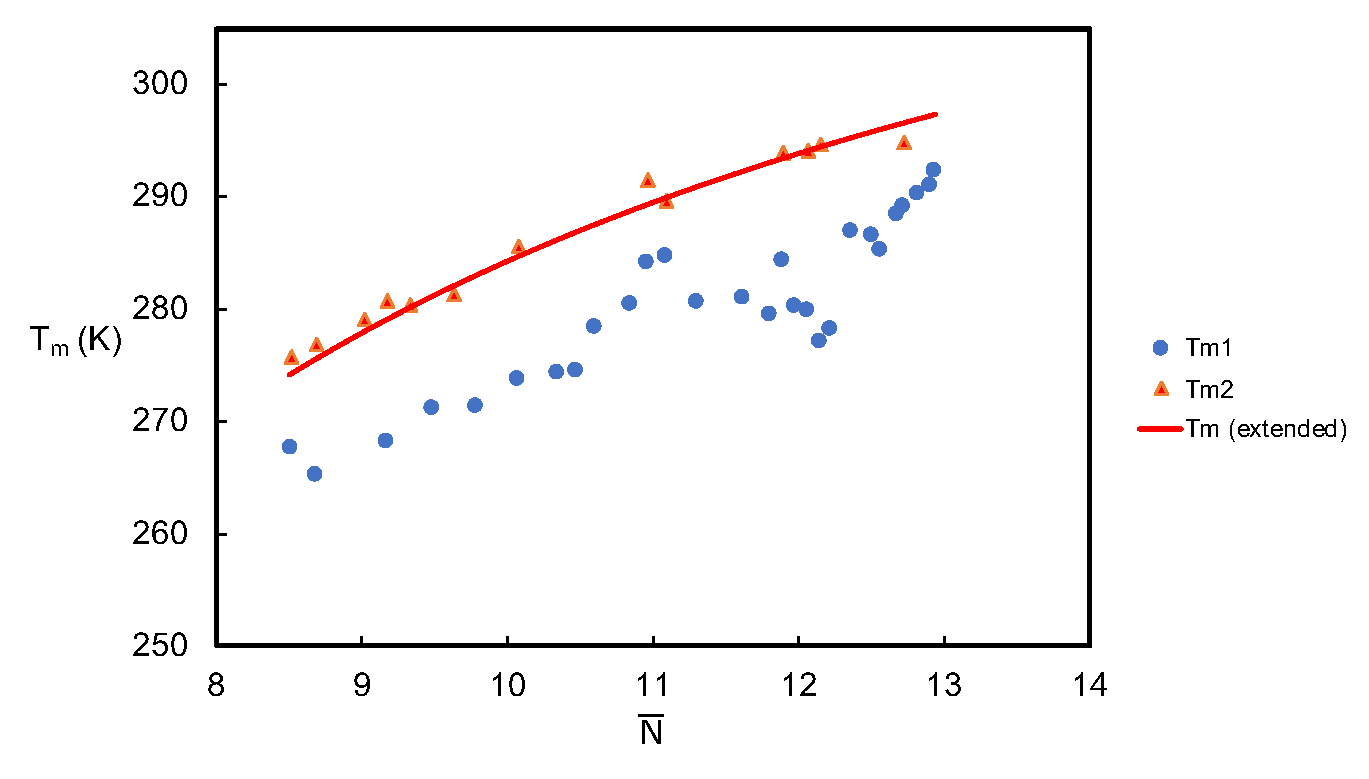
\includegraphics[width=\linewidth]{fitTm1}
\caption{$T_{m1}$ data fitting to Gibbs Thomson equation.}
\label{fig:fitTm1}
\end{figure}

For the lower melting points, which correspond to once-folded chains, the chains emanating from the lamella enter the amorphous phase to make a fold, and then re-enter the lamella. In this case we suppose that it takes $N_{a}$ monomers for a single chain to complete this turn, instead of bending $180^\circ$ sharply. This conformation has two chain-end monomers on one side of the lamella, and $N_{a}$ monomers on the fold on the other side, which enables us to calculate the interfacial tension $S_{1-fold}$ as:

\begin{equation}
\label{eqn_S1fold}
S_{1-fold} = \dfrac{2S_{ext} + N_{a} S_{folds}}{2 + N_{a}}
\end{equation}

With $S_{1-fold}$ obtained, the value of $N_{a}$ is now the only free parameter that could be tuned to fit the lower melting points with Gibbs Thomson equation. From the curve fitting (Figure \ref{fig:fitTm2}), $N_{a}$ is determined to have a value of 3.5. For a PEO chain, this is approximately 2.6 times its persistence length \cite{Takahashi1973}, which suggests that this chain conformation is a possible and reasonable model of chain-folding.

\begin{figure}[H]
\center
\vspace{1 cm}
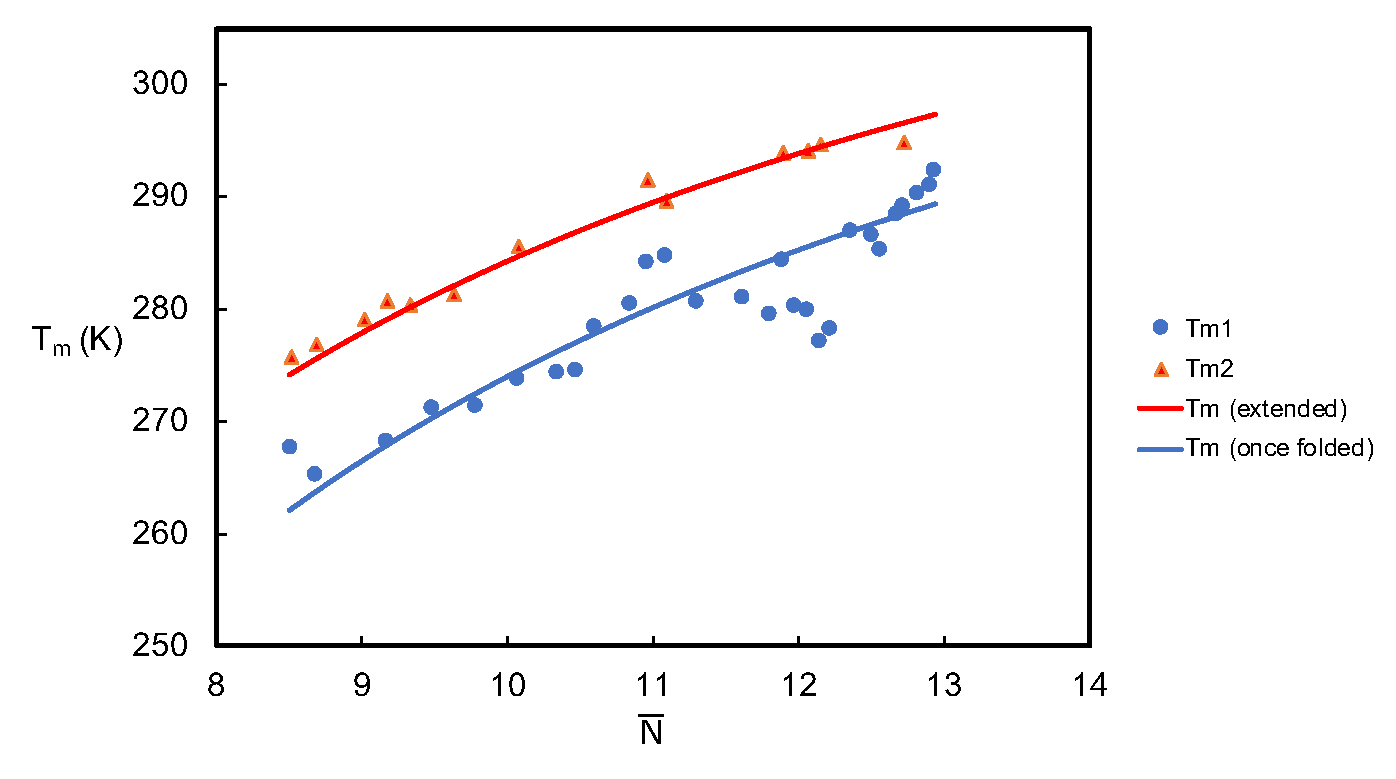
\includegraphics[width=\linewidth]{fitTm2}
\caption{$T_{m1}$ and $T_{m2}$ data fitting to Gibbs Thomson equation.}
\label{fig:fitTm2}
\end{figure}

In the plots of melting temperatures, the x-axis, $\bar{N}$, is the number average value of all the composing $N$'s in each fraction, characterized directly with MALDI or interpolated based on the MALDI data. However, only with single integer $N$ values could we be able to talk about the melting temperatures given by the Gibbs Thomson curves. For a mixtures of different $N$'s, its melting temperature potentially lies anywhere within the range of $T_{m}$'s of its composing $N$'s. A more careful way to present our chain-folding models together with the $T_{m}$ data would be as Figure \ref{fig:fitTm} shows. Dashed boxes are generated for each $T_{m}$ curve, with the top (bottom) of the box representing the melting point of the highest (lowest) $N$ value present in any potential purified fraction lying on the curve in this particular box. In generating the bars, $N$ components with a percentage less than 5 \% are neglected. Notice that each curve passes through all of the corresponding boxes, with only several data points falling outside.

\begin{figure}[H]
\center
\vspace{1 cm}
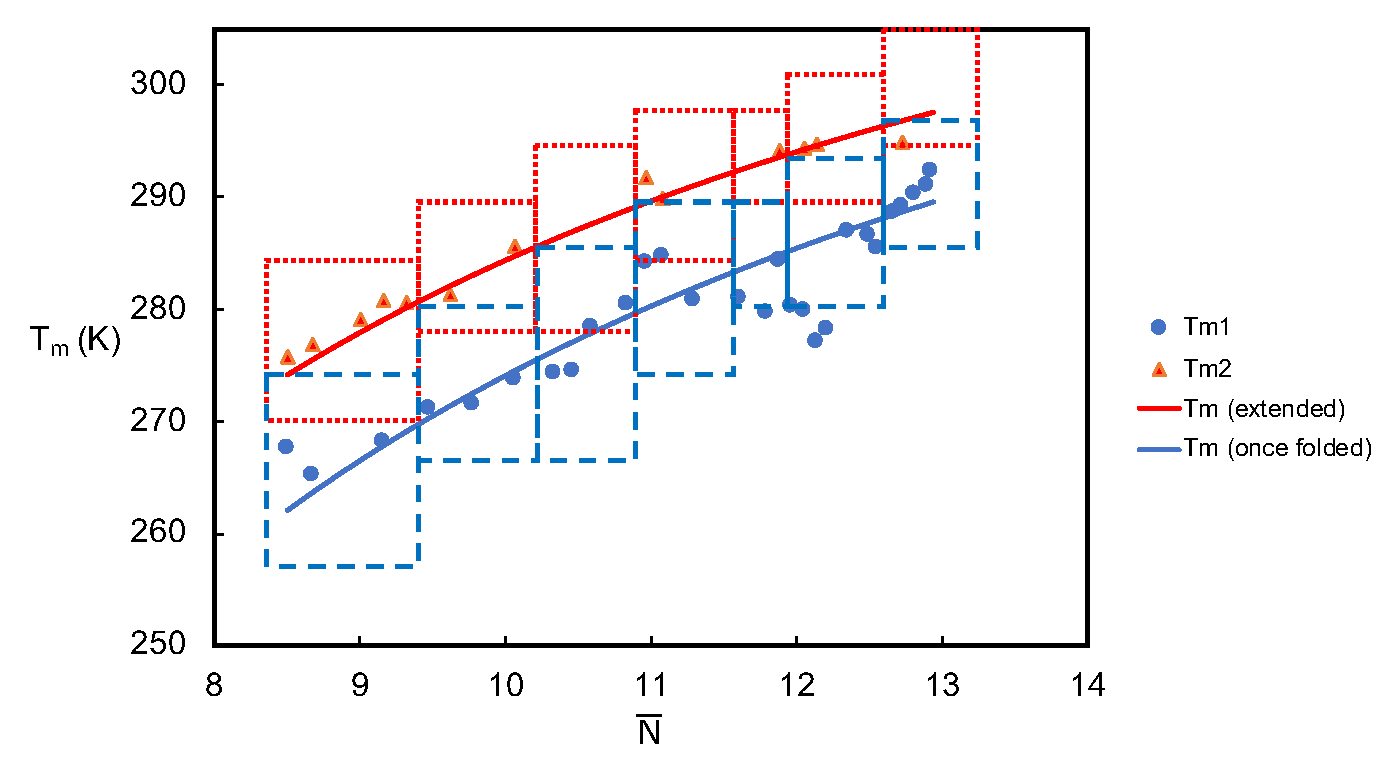
\includegraphics[width=\linewidth]{fitTm}
\caption{Gibbs Thomson relation fitting with potential range bars on $T_{m}$ data points.}
\label{fig:fitTm}
\end{figure}

\subsubsection{Comparison to N-alkanes}

As mentioned previously, PEO is a polymer with linear structure, as well as N-alkanes. Therefore, some comparisons to N-alkanes are necessary to better understand the phenomena and properties we have observed.

Before the lamellar structure of PEO was discovered, N-alkanes had been revealed to form "single crystal platelets", with chain ends at surfaces of these lamellae \cite{Richardson1965}. The thickness of each lamella is around 100 \AA, while it could vary from 60-80 \AA  to up to 150 \AA, depending on certain conditions \cite{Keller1957a}. In order for long chains whose extended length is larger than this thickness to accommodate in such a layer, polymers are found to fold back and forth in the layer. Depending on the length of chains, they need to fold for different times in the lamellae. For N-alkanes, the lower molecular weight limit for fold-chain conformation is 2100 $g/mol$, or 150 carbon atoms in the chain, equivalently \cite{Ungar1986}. For crystallization from solutions, this limit is slightly lower than that from the melt, but still similar \cite{Alamo1993}.

It was further discovered that for long N-alkanes, the fold length (lamella thickness) is a function of crystallization temperature $T_{c}$. When the supercooling is small, lamellae are grown with larger thickness \cite{Ungar1986}. 

The number of folds for each polymer chain was at first believed to be quantized, i.e., the chains could only take integer number of folds in the lamella, or they exist as extended chains \cite{Ungar1986}. Kovacs \textit{et al} obtained same results for PEO oligomers as well, where only integer folds are allowed \cite{Kovacs1977}. However, it was later discovered that non-integer folds (NIF) are also possible to be present. Real-time small-angle X-ray scattering (SAXS) experiments \cite{Zeng1998} revealed that at early stages of crystal formation, long alkane chains form NIF crystals. The amorphous layers in between of lamellae of NIF crystals have a thickness of 6 to 8 nm, which are much looser than that of extended chain crystals. During crystallization process, NIF lamellae further thicken or thin until the thickness reaches integral fractional (IF) values of the extended chain length, through refolding of chains. The amorphous layers then become denser and the folds turn sharper, corresponding to a more stable state of the crystal \cite{Ungar1986}.

Richardson \cite{Richardson1965} studied single crystal polyethylene with adiabatic calorimeter, in order to investigate the folding and chain re-entry in the lamellae. Chains exiting the crystalline layer may return to themselves immediately, as suggested in the adjacent re-entry model in Section \ref{sec: folded chain model}, or they may float in the amorphous region, and return the lamellae from a further site, resulting in a loose fold. From the result of calorimetry and small-angle X-ray experiments, the number of carbon atoms involved in each sharp fold in the adjacent re-entry model is found to be six, which is three monomers for polyethylene. In comparison to our crystallization analysis for PEO, this number is close to the result we obtained, which is 3.5 monomers on each fold.

\subsubsection{Fractionation of chains during crystallization}

In the DSC measurements, fractionation of chains with different $N$'s is sometimes observed. During some of the repeated DSC measurements, several samples show double melting peaks (an example shown in Figure \ref{fig:3K difference}), with both melting temperatures near the same $T_{m}$ curve. The two peaks are separated by around 3 K, which is likely the difference between the melting temperatures of two neighboring $N$'s according to our calculation, rather than the difference between the two chain conformations (extended and folded). It is worth noting that this fractionation is more commonly observed at the higher $T_{m}$ than at the lower $T_{m}$, because in the extended conformation, the crystal lamellae composing of two neighboring $N$'s have a large difference in thickness than in the folded conformation.

\begin{figure}[H]
	\center
	\vspace{1 cm}
	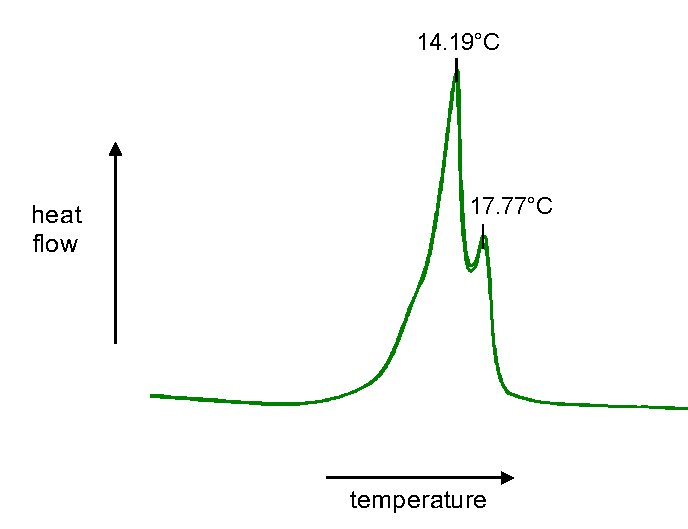
\includegraphics[width=0.5\linewidth]{doublepeaks3K}
	\caption{Part of DSC curve (melting) from regular run on $\bar{N} = 11$.}
	\label{fig:3K difference}
\end{figure}

\subsubsection{Tuning chain-folding mode}

Most of the fractions show two melting points in DSC measurements, while some of the fractions only shows one, lying either on the $T_{m1}$ curve or the $T_{m2}$ curve. For the fractions where when the higher $T_{m}$ is observed, on the DSC cooling ramp there are usually two crystallization peaks, suggesting that the polymers still form both extended chains structure and folded chains structure, but before increasing to the melting temperature, once-folded chains relax themselves and recrystallize into extended form. However, when the lower $T_{m}$ is observed, on the cooling ramp there is only one crystallization peak. This is an indication that the cooling rate during crystallization may not have been slow enough for the chains to crystallize in the extended form.

The following treatment (Figure \ref{fig:treatment}) is then applied to further verify our observation. With some of the fractions that show the lower $T_{m}$ (either with or without the higher $T_{m}$) in normal DSC measurements, we keep the sample at a temperature between $T_{m1}$ and $T_{m2}$ for a time long enough to melt all the once-folded chains and leave all the extended chains. Then we cool the sample to a much lower temperature, and measure its melting again. During the second DSC measurement only the higher $T_{m}$ appears, which is a direct validation that we have successfully forced the once-folded chains to recrystallize into extended chains by applying the treatment. Figure \ref{fig:DSC before and after} is an example measurement we did on purified fraction with $N = 12.3$.

\begin{figure}[H]
\center
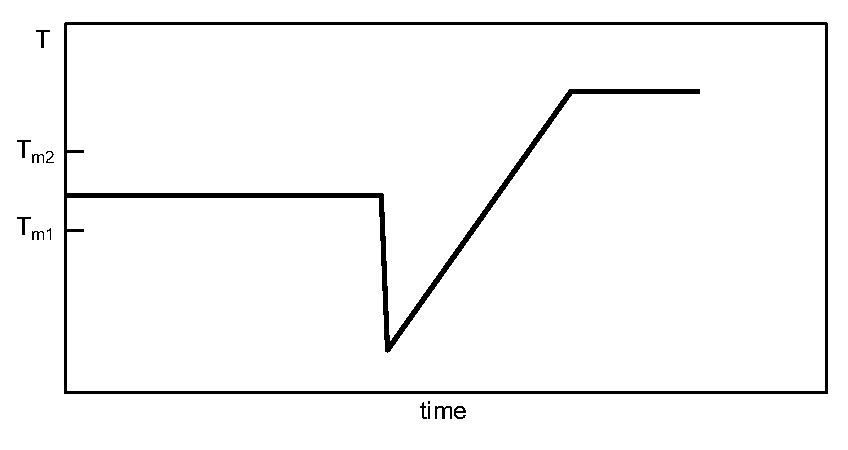
\includegraphics[width=0.6\linewidth]{treatment}
\caption{Thermal treatment on products with a lower $T_{m}$ present.}
\label{fig:treatment}
\end{figure}

\begin{figure}[H]
	\centering
\begin{subfigure}[b]{0.6\linewidth}
	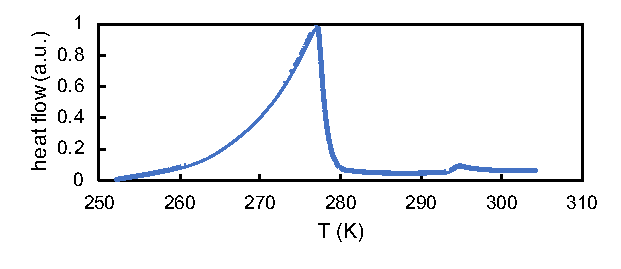
\includegraphics[width=\linewidth]{DSCbefore}
	\caption{Before thermal treatment there is a major melting transition peak followed by a small peak.}
\end{subfigure}
\begin{subfigure}[b]{0.6\linewidth}
	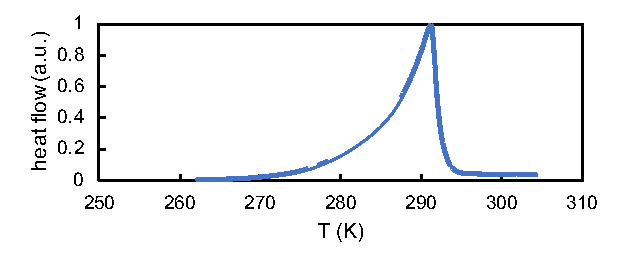
\includegraphics[width=\linewidth]{DSCafter}
	\caption{After thermal treatment only one melting peak near $T_{m2}$ is observed.}
\end{subfigure}
\caption{DSC measurements on purified fraction with $N = 12.3$ before and after thermal treatment.}
\label{fig:DSC before and after}
\end{figure}

\subsubsection{Comparison between purified fractions and neat sample}

When we compared the DSC curves of the neat sample and the purified fractions, surprisingly we noticed that some of the fractions performed unexpected melting behaviors, as Figure \ref{fig:neatvsfractions} shows. From the curves of some products from early stages of evaporation, we expect that in the neat mixed sample they should start melting at temperatures much lower than the observed melting temperature of the neat sample. However, this is not what happens. According to this phenomenon, we believe that when the short chains are mixed with longer chains, they become influenced and perform different crystallization behaviors than in a more monodisperse sample. One of the possible explanations to this is that in the presence of longer chains, the shorter chains tend to act as amorphous phase, even at temperatures lower than the melting points of themselves. As a matter of fact, it is also possible that the short chains only take up a very small portion (fractions with $N \leq 10$ are 14\% of the neat sample) in the neat sample, therefore the heat flow signal from them could easily be overwhelmed by that of major components.

\begin{figure}[H]
\center
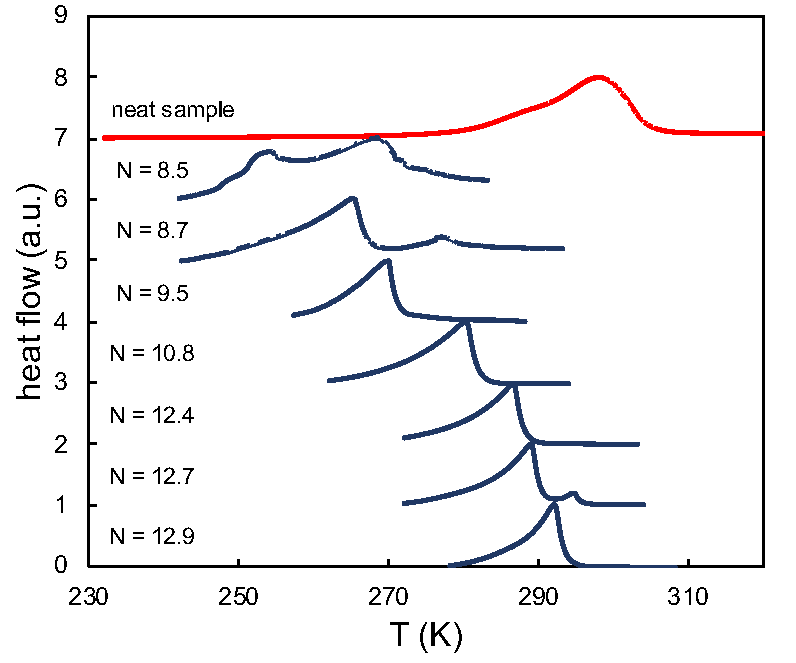
\includegraphics[width=0.8\linewidth]{neatvsfractions}
\caption{DSC curves of the neat sample (red) and some of the purified fractions (blue).}
\label{fig:neatvsfractions}
\end{figure}

\subsubsection{End-group effects}

In \ref{Tm and Yeates}, we reviewed Yeates' study on melting of monodisperse and polydisperse PEO oligomers. Now we would like to compare our results for purified fractions with theirs. Surprisingly, it turns out that the melting temperatures we obtained agree more with the polydisperse samples in their measurements. This could be an indication that the melting points difference they observed between the monodisperse and polydisperse samples is very unlikely to be due to polydispersity. Instead, it could be related to specific properties such as end-group chemistry.

End-group effects on PEO crystallization has been studied by many researchers and it has been found that the type of end-groups directly influences properties including melting temperature and crystallinity, as shown in Table \ref{tab:end-group effects}. Monodisperse PEO with hydroxy end-groups has been reported to display different crystallinities and $T_{m}$'s than that with methoxy end-groups. The difference in crystallinity is believed to be due to different heats of interaction related to the end-groups at the lamellar surfaces. The difference in melting temperature is attributed to different environments at a crystalline lamellar surface and in melt, because lamellar surfaces are much more ordered compared to the melt, which magnifies the effect of end-groups on the surfaces, while in a melt environment, the effect of end-groups could be hidden in the melt background. Polydisperse PEO samples with different end-groups, however, display different crystallinities but similar $T_{m}$'s. It is argued that rejection of methoxy end-groups from the lamellar surfaces results in higher entropy of the crystal, leading to a lower enthalpy of melting, and a lower crystallinity. In terms of the melting temperature, it is claimed that the disordered lamellar surface and the melt have similar environments, so the effect of end-groups on $T_{m}$'s would appear less significant.
\begin{table}[H]
\centering
	\begin{tabular}{ |c|c|c|c| } 
		\hline
		 & monodisperse PEO & polydisperse PEO \\
		\hline
		\hline
		crystallinity & different & different \\ 
		\hline
		$T_{m}$ & different & similar \\ 
		\hline
	\end{tabular}
	\caption{\label{tab:end-group effects}Comparison of PEO with hydroxy and methoxy end-groups \cite{Marshall1981}.}
\end{table}
In our experiments, the PEO samples only contain hydroxy end-groups, while in Yeates' study, the synthesis of monodisperse samples involved end-groups containing sulfur. Based on the evidences and analysis mentioned above, the  disagreement between our results and theirs could be that sulfur results in different interaction energy with the crystalline layer, and potentially led to different melting temperatures. From literature it is found that sulfur decreases the interfacial tension of liquid iron with $\text{Al}_{\text{2}}\text{O}_{\text{3}}$ \cite{Halden1955}, and also decreases the interfacial energy between Fe-C melt and graphite \cite{Jung2005}. However, no direct measurement results have been found in terms of the effect of sulfur-containing end-groups on the interfacial energy and melting temperature of a polymer.

\subsection{Degree of crystallinity}

PEO has been know as a polymer with high crystallinity due to its linear structure. However, based on the fact that polymers almost never crystallizes completely, it is of interest to study the degree of crystallinity $X_{c}$ of our samples. We determine $X_{c}$ of the products from the heat of fusion $\Delta H_{f} (T_{m})$ on melting in DSC measurements. The heat of fusion could be calculated from the area under the melting peak, and the degree of crystallinity is defined as \cite{Kong2002}:

\begin{equation}
\label{eqn_Xc}
X_{c} = \dfrac{\Delta H_{f} (T_{m})}{\Delta H_{f}^{0} (T_{m}^{0})}
\end{equation}

\noindent
where $X_{c}$ is the degree of crystallinity by weight fraction, $\Delta H_{f} (T_{m})$ is the enthalpy of melting transition, and $\Delta H_{f}^{0} (T_{m}^{0})$ is the enthalpy of melting of PEO with 100 \% crystallinity \cite{Yave2010}. By integrating the melting peaks on the DSC curves, we obtain $X_{c}$ of the purified products, as shown in Figure \ref{fig:Xc}.

\begin{figure}[H]
\center
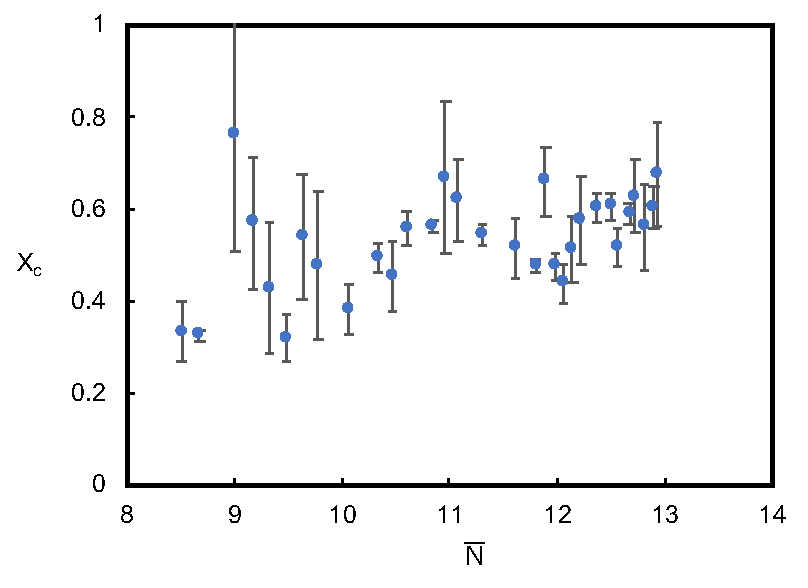
\includegraphics[width=0.7\linewidth]{Xc}
\caption{Degree of crystallinity of purified products.}
\label{fig:Xc}
\end{figure}

It is easily noticed from the figure that our data is not precise enough since the error bars for some of the fractions are quite large. This results from the deviation (0.1 mg) of the scale used to weigh the samples. The enthalpy of melting $\Delta H_{f} (T_{m})$ calculated from the DSC curve is directly related to the weight of sample, and for samples with a small weight, the deviation is comparable to its weight. Therefore, for more precise data of $X_{c}$, larger amount of sample is required, which brings forward the demand for technical improvements including scaling-up of our evaporative purification system.

We would also like to compare our results of PEO crystallinity with other studies, as shown in Figure \ref{fig:Xc comparison}. Although there is a limited number of measurement results on PEO crystallinity with such low $\bar{N}$ values, most of our results lie in the range of several other studies in the literature.

\begin{figure}[H]
	\center
	\vspace{1 cm}
	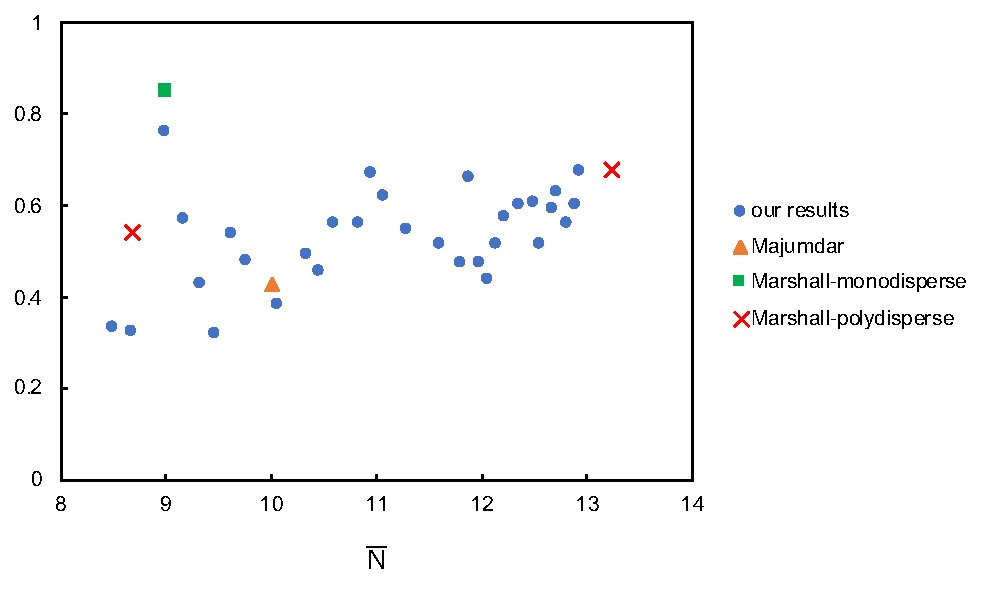
\includegraphics[width=0.9\linewidth]{Xccomparison}
	\caption[Comparison of degree of crystallinity measured in different studies]{Comparison of degree of crystallinity measured in different studies. Majumdar: data from "Physical characterization of polyethylene glycols by thermal analytical technique and the effect of humidity and molecular weight" by R Majumdar \textit{et al}, \textit{Pharmazie}, 65:343-347, 2010 \cite{Majumdar2010}. Marshall: data from "Crystallinity of Ethylene Oxide Oligomers" by A Marshall \textit{et al}, \textit{Eur. Polym. Journal}, 17(893), 1981. \cite{Marshall1981}.}
	\label{fig:Xc comparison}
\end{figure}

An interesting fact about the $X_{c}$ data is that when we bring Figure \ref{fig:Xc} and Figure \ref{fig:Tm} into comparison (even though $X_{c}$ and $T_{m}$ are not directly related), it could be noticed that they have a similar trend, especially with the bump pattern located at $\bar{N}$ around 11. However, the reason behind this observation is still unclear to us and needs further investigation.

\chapter{Crystal growth review and measurements}\label{chap_growth}
\graphicspath{{./growth/graphs/}}

In the previous chapter we discussed about the thermodynamics of polymer crystallization, while this process is in fact controlled by kinetics more than thermodynamics due to the nature of polymers. Kinetic theories typically analyze a process from two aspects: "driving force" and "free energy barrier" \cite{Zhang2016a}. "Driving force" in the case of polymer crystallization refers to the free energy difference between the crytalline state and the amorphous state, and "free energy barrier" includes all kinds of factors that are against the crystallization process, such as entanglement of chains, defects in the system, etc. These two factors compete with each other, and the system reaches the most stable state based on the balance of them.

\section{Crystallization with spherulites}

When the polymer crystal is grown from a melt, superstructures called spherulites are normally formed. These structures are composed of stacked lamellae that have grown from a common center, as shown in Figure \ref{fig:spherulite}. Spherulites are normally formed when there is no thermal gradient present, because in the presence of thermal gradient with a certain direction, crystal growth would follow the gradient instead of growing radially \cite{Carraher2003}. In the spherulites, polymer chains are aligned perpendicular to the radius of the spherulites. During crystallization, the spherulites grow until they contact each other, and their sizes range from microns to millimeters \cite{Vasile2000}, which could be easily observed under an optical microscope. Among the crystalline stacks are amorphous regions, together forming a semicrystalline structure.

\begin{figure}[H]
\center
\vspace{1 cm}
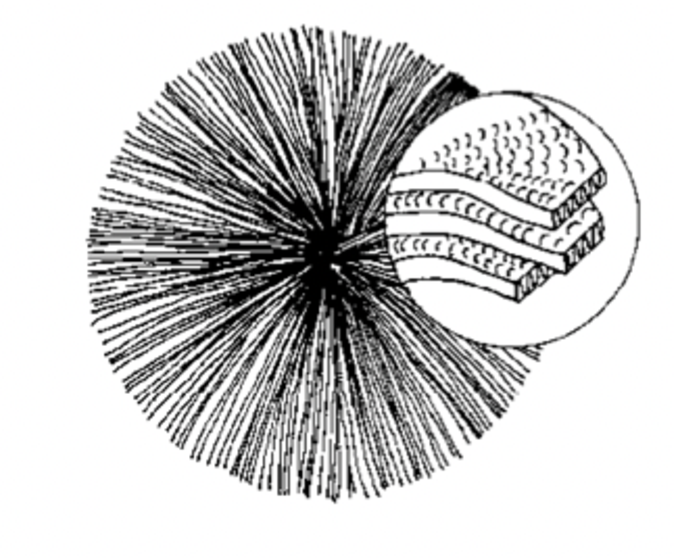
\includegraphics[width=0.5\linewidth]{spherulite}
\caption[A polymer spherulite with folded-chain lamellae.]{A polymer spherulite with folded-chain lamellae \cite{High}.}
\label{fig:spherulite}
\end{figure}

The growth of a spherulite is controlled by many factors including the number of nucleation sites, polymer structure, crystallization temperature, cooling rate, etc. For example, when the crystallization temperature is low enough or there are a large number of present nuclei, many spherulites would be created and grow into relatively small sizes; while if the supercooling is small, and fewer nuclei are present, fewer spherulites would form, but they are larger in size \cite{LindaSawyerDavidT.Grubb2008}. Spherulites are optically anisotropic because of the alignment of the linear polymer chains. When they are viewed under an optical microscope, with crossed polarizers on, certain patterns such as Maltese cross consisting of eight alternating bright and dark fan-shaped areas (Figure \ref{fig:Maltese cross}) are often observed, resulting from the birefringence of the lamellae \cite{Bower2002}.

\begin{figure}[H]
\center
\vspace{1 cm}
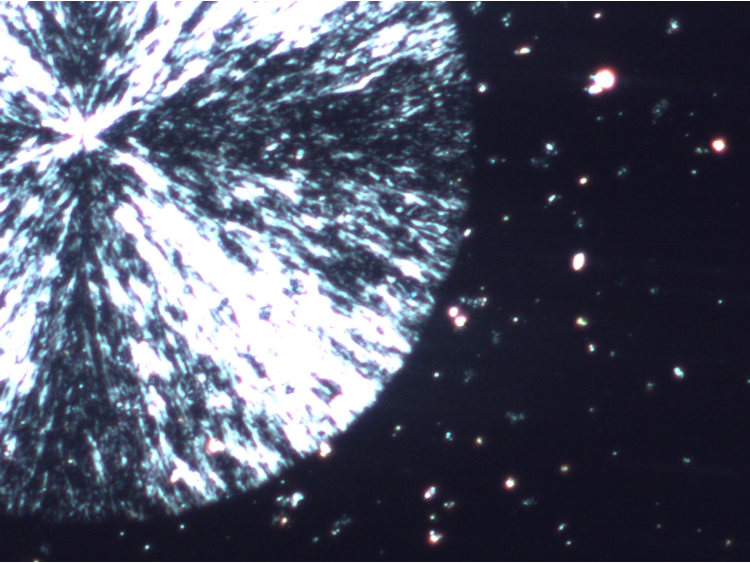
\includegraphics[width=0.5\linewidth]{Maltese}
\caption{Optical microscope image (with crossed polarizers on) of fraction with $\bar{N} = 12.4$ at 260.65 K.}
\label{fig:Maltese cross}
\end{figure}

\subsection{Nucleation} \label{nucleation}

Crystallization process can be divided into two stages: nucleation and crystal growth. Nucleation is the primary step in the crystallization of a polymer. As temperature decreases, a polymer normally does not crystallize immediately when it reaches the melting temperature, but rather needs a considerable supercooling before crystallization. The reason is that crystallization starts with nucleation, and if the polymer sample has little or no nuclei present, the temperature needs to be kept decreasing until the sample grows a nucleus out of itself, which is called primary nucleation. The driving force of this process is the local density fluctuation, and it could occur in the range of below melting temperature and above glass transition temperature.

Apart from primary, there are also secondary and tertiary nucleation. If we consider the formation of a cubic nucleus, primary nucleation requires 6 new faces to be formed, while secondary nucleation requires 4 new faces (on the surface of present nuclei), and tertiary nucleation requires only 2 new faces (at the edge of present nuclei) \cite{Chai2016}.

Primary nucleation is further classified into homogeneous nucleation and heterogeneous nucleation. Homogeneous nucleation refers to a nucleation process that is purely induced by thermal fluctuations and does not involve the influence of any solids, including present crystal, container walls, or foreign particles present in the crystallizing sample. Heterogeneous nucleation, however, refers to a primary nucleation with the help of impurity particles, either uncontrolled or deliberately introduced into the sample \cite{Strobl2007}. Homogeneous nucleation would be mainly focused on here, but heterogeneous nucleation is much more common in real cases. Foreign particles help greatly reduce the free energy barrier of the phase transition from liquid to crystal, and lead to a smaller supercooling.

In a homogeneous nucleation process, thermal fluctuations result in the formation of embryos (small aggregates with enhanced inner order), and the size of the embryos determines if they could survive through the energy barrier and grow into a larger crystal. If the embryo is not big enough, there would only be a small free energy loss caused by crystallization, compared to the free energy barrier in creating the embryo surfaces. In this case, the embryo could not survive and has to melt. Assuming the embryos are spherical, here we could use classical nucleation theory to derive the critical size of an embryo \cite{Chai2016}.

The total free energy of an embryo is:

\begin{equation}
\label{eqn_delta G of embryo}
\Delta G = -\dfrac{4}{3} \pi r^{3} \Delta g + \sigma_{e} 4 \pi r^{2}
\end{equation}

\noindent
where $r$ is the embryo radius, $\Delta g$ is the free energy per unit mass on melting, and $\sigma_{e}$ is the surface free energy of the embryo.

The plot of $\Delta G$ vs $r$ is shown as Figure \ref{fig:Delta G embryo}. We notice there is a maximum in  $\Delta G$, $\Delta G^{*}$, for a critical $r$ value, $r^{*}$. Below this value, $\Delta G$ increases with $r$, while after surpassing it, $\Delta G$ decreases as $r$ increases. When the thermal fluctuations are strong enough to produce embryos larger than $r^{*}$, the embryos could then grow into crystals. These two critical values could be calculated \cite{Hoffman1997} from Equation \ref{eqn_delta G of embryo}:

\begin{equation}
\label{eqn_critical radius of embryo}
r^{*} = \dfrac{2\sigma_{e}}{\Delta g}
\end{equation}

\begin{equation}
\label{eqn_critical energy of embryo}
\Delta G^{*} = -\dfrac{16\pi\sigma_{e}^{3}}{3\Delta g^{2}}
\end{equation}

\begin{figure}[H]
\center
\vspace{1 cm}
\begin{tikzpicture}
\begin{axis}[
    ticks=none,
    axis x line=middle,axis y line=left,
    xlabel = {$r$},
    ylabel = {$\Delta G$},
    ymin=-0.121,ymax=0.2,ylabel style={rotate=-90},
]
\addplot [
    domain=0:1.1, 
    range=-0.121:2
    samples=100, 
    color=blue,
]
{x^2 - x^3};
%\draw [ultra thick, dotted, draw=red] 
%        (axis cs: 0,4/27) -- (axis cs: 2/3,4/27);
%\draw [ultra thick, dotted, draw=red] 
%        (axis cs: 2/3,0) -- (axis cs: 2/3,4/27);
%\node[label={180:{($r^{*}$,$\Delta G^{*}$)}},circle,fill,inner sep=2pt] at (axis cs:2/3,4/27) {};
\addplot[mark=*] coordinates {(2/3,4/27)} node[pin=150:{$r^{*}$,$\Delta G^{*}$}]{} ;
\end{axis}
\end{tikzpicture}
\caption{Total free energy of an embryo $\Delta G$ vs embryo radius $r$, where $r^{*}$ and $\Delta G^{*}$ are the critical radius and the critical free energy, respectively.}
\label{fig:Delta G embryo}
\end{figure}

Intuitively we would expect both $r^{*}$ and $\Delta G^{*}$ to be in negative correlation with the extent of supercooling $\Delta T$, and in fact this could be proved. Similar to what we assumed in \ref{Thermodynamics of polymer crystallization}, here we assume that the enthalpy and entropy do not vary significantly near the crystallization temperature. Therefore, from

\begin{equation}
\label{eqn_Delta g at Tm}
\Delta g(T_{m}) = \Delta h(T_{m}) - T_{m}\Delta s(T_{m}) = 0
\end{equation}


\begin{equation}
\label{eqn_Delta g at Tc}
\Delta g(T_{c}) = \Delta h(T_{c}) - T_{c}\Delta s(T_{c}) = 0
\end{equation}

\noindent
we have

\begin{equation}
\label{eqn_Delta g Tc}
\Delta g(T_{c}) = \Delta h(T_{c}) - T_{c} \dfrac{\Delta h(T_{c})}{T_{m}} = \Delta h(T_{c}) \dfrac{T_{m} - T_{c}}{T_{m}} = \Delta h(T_{c}) \dfrac{\Delta T}{T_{m}}
\end{equation}

In consistency with the case of embryo growth, we rewrite it as

\begin{equation}
\label{eqn_Delta g of embryo}
\Delta g = \Delta h \dfrac{\Delta T}{T_{m}}
\end{equation}

Based on Equations \ref{eqn_critical radius of embryo} and \ref{eqn_critical energy of embryo}, we obtain the following relation:

\begin{equation}
\label{eqn_relation for r}
r^{*} \propto \Delta T^{-1}
\end{equation}

\begin{equation}
\label{eqn_relation for G}
\Delta G^{*} \propto \Delta T^{-2}
\end{equation}

As the crystallization temperature ($T_{c}$) gets lower, corresponding to a larger supercooling $\Delta T$, $r^{*}$ and $\Delta G^{*}$ gets smaller, which means an easier nucleation. In addition, according to the nucleation theory by Turnbull and Fisher \cite{Turnbull1949}, the nucleation rate, $i$, is expressed as:

\begin{equation}
\label{eqn_nucleation rate}
i = i_{0}exp(- \dfrac{\Delta E + \Delta G^{*}}{k T})
\end{equation}

\noindent
where $i_{0}$ is a pro-exponent factor, $\Delta E$ is the nucleation activation energy, and $\Delta G^{*}$ is the critical nucleation energy. The dependence on $\Delta T$ through $\Delta G^{*}$ suggests that the nucleation rate $i$ is higher for a larger supercooling, and thus a faster nucleation. However, we need to be careful that when temperature decreases to near the glass transition temperature, $T_{g}$, chain mobility is highly restricted, which makes it harder for thermal fluctuations to produce nuclei. Therefore, there exists a maximum nucleation rate at a temperature between $T_{g}$ and $T_{c}$.

Nucleation process could be described by nucleation time $\tau _{nuc}$ as well, which is simply the inverse of nucleation rate, and could be directly measured. Nucleation rate is significantly slower than crystal growth rate, especially for homogeneous nucleation, which makes it very convenient to measure these two processes separately. In a study \cite{Massa2004} of homogeneous nucleation in PEO crystallization, the relation between $\tau _{nuc}$ and the volume of the crystallizable droplets $V$ was shown. Impurity-free discrete PEO droplets are formed through dewetting on a polystyrene film, and cooled under optical microscopy with crossed polarizers on to observe the nucleation of each droplet. Figure \ref{fig:tauV} demonstrates their findings.

\begin{figure}[H]
\center
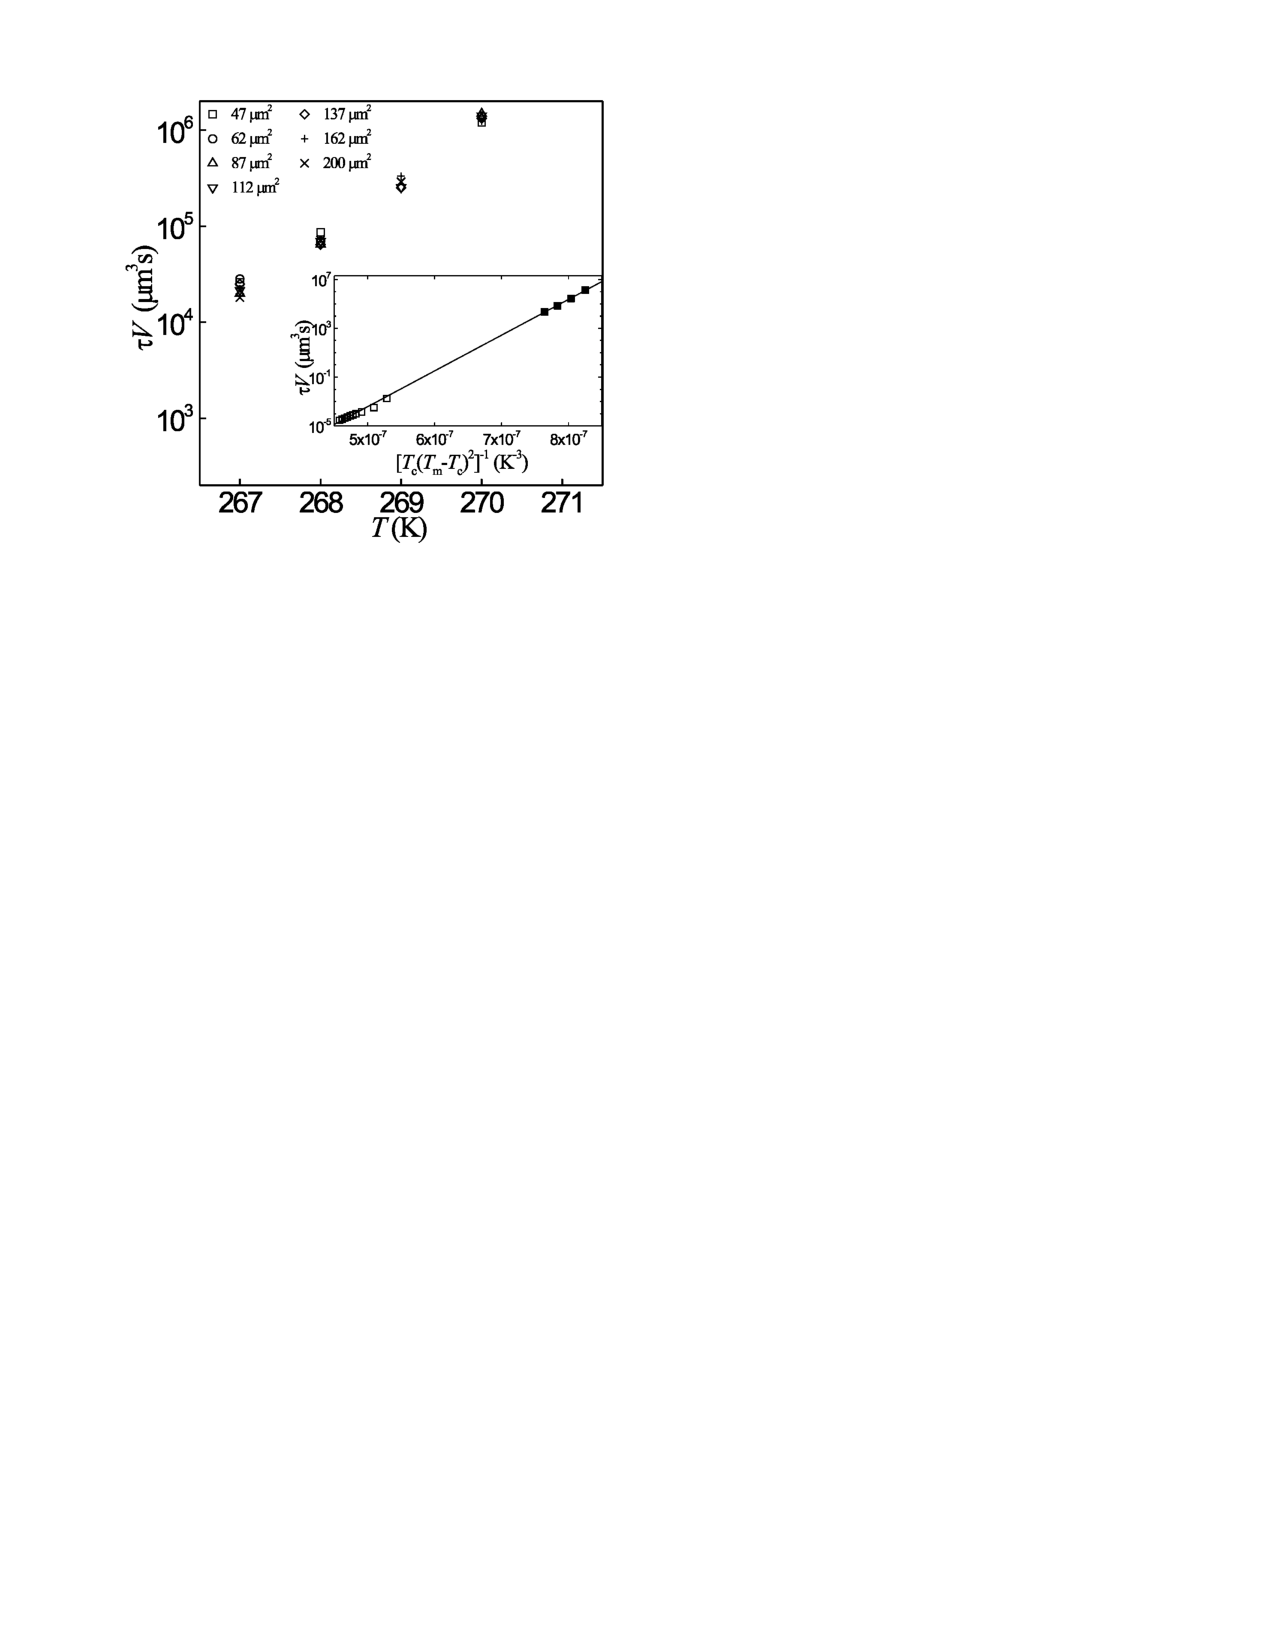
\includegraphics[width=0.6\linewidth]{tauV}
\caption[Volume-normalized time constant, $\tau V$, as a function of temperature.]{Volume-normalized time constant, $\tau V$, as a function of temperature \cite{Massa2004}. In the index the averaged dewetted droplet data (solid symbols) are in agreement with data from \cite{Rottele2003} (open symbols), both with linear dependence on $[T_{c}(T_{m}-T_{c})^{2}]^{-1}$ as expected from classical nucleation theory \cite{Strobl2007}.}
\label{fig:tauV}
\end{figure}

The observation results show that

\begin{equation}
\label{eqn_nucleation time}
\tau _{nuc} \propto V^{-1}
\end{equation}

At the same crystallization temperature, droplets with different volumes have the same value of the volume-normalized time constant, $\tau V$, and it decreases (meaning increasing rate) exponentially as the supercooling becomes larger. The close agreement between these two sets of data and their huge difference ($\sim 8$ orders of magnitude) in $\tau V$ suggests that nucleation mechanism is consistent within a huge range of size. The many differences in these two experimental systems indicates that nucleation is dominated by the bulk rather than the surface.

\subsection{Crystal growth}

After nuclei have been formed, some of them could grow into larger crystals by adsorbing crystallizable materials. Crystal growth is either diffusion-controlled or interface-controlled.

Crystals growing from dilute solutions are typically diffusion-controlled, since in such cases the growth rate depends on the diffusion rate of crystallizable materials onto the surfaces of present nuclei. According to Fick's diffusion law \cite{Fick1855,FickZiirich1995}, the relation between the radius of a crystal $r$ and time $t$ has been found to be \cite{Ouyang1998,Ouyang1999,HaoOuyang2004,Naga2013}:

\begin{equation}
\label{eqn_diffusion crystal radius}
r \propto t^{\frac{1}{2}}
\end{equation}

When the solution concentration is high, or when the crystal is growing from a melt, diffusion rate is no longer the limiting factor in its growth, because nuclei are surrounded by sufficient crystallizable materials. Therefore, it depends more on the process of crystallizable materials attaching onto existing nuclei. In describing the attachment and the formation of crystal lamellae, there is one widely-accepted theory proposed by Lauritzen and Hoffman \cite{Lauritzen,Hoffman,Lauritzen1973}. It builds a connection between microscopic movements and macroscopic quantities, and has become the most successful theory to describe this process, although it has also been criticized by some researchers saying that it oversimplifies crystal growth by applying a mean field description \cite{Zhang2016a}.

Lauritzen-Hoffman (LH) theory treats crystal growth as a secondary nucleation process, and one of the basic assumptions is that the nucleus is in fact a single stem grown from thermal fluctuations. It then acts as a growth front, and other stems deposit onto its surface and crystallize stem by stem into a lamella, thus creating a new layer through lateral spreading. When the present surface layer is taken up, this spreading process is repeated if another nucleus is formed on top of this layer.

In order to quantify this process, four parameters need to be defined: the surface nucleation rate, $i$; lateral covering rate, $g$; perpendicular growth rate, $G$; the length of surface, $L$. Three regimes are predicted in the model, as shown in Figure \ref{fig:LH theory}.

\begin{figure}[H]
\center
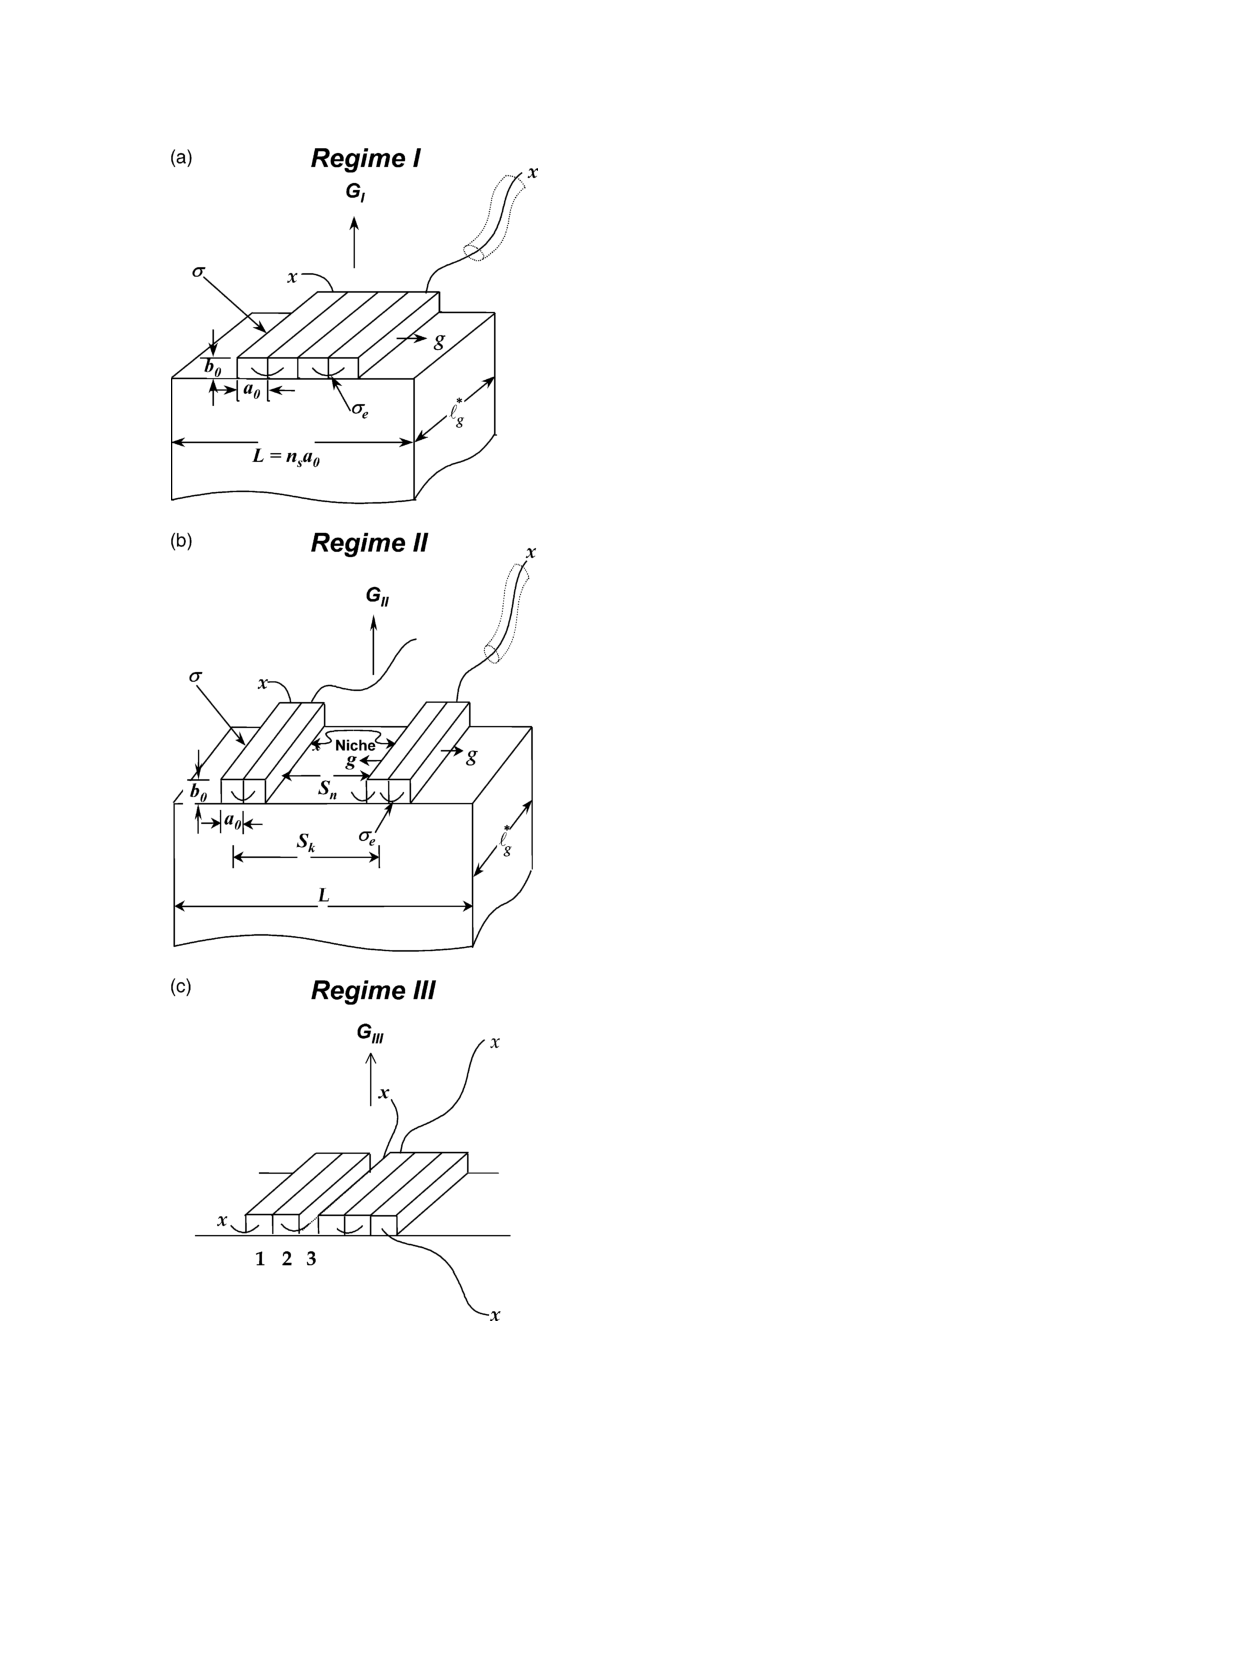
\includegraphics[width=0.4\linewidth]{LHtheory}
\caption[Polymer crystal growth in three regimes in LH theory.]{Polymer crystal growth in three regimes in LH theory \cite{Cheng2005}.}
\label{fig:LH theory}
\end{figure}

In regime \Romannum{1}, $\Delta T$ is low, and according to the nucleation theory \cite{Turnbull1949} mentioned in \ref{nucleation}, nucleation rate $i$ is low. In the case where $i$ is smaller than $g$, there is enough time for polymer chains to cover the entire surface, since this process is restricted by $i$. The growth rate in this regime is given by

\begin{equation}
\label{eqn_regime1}
G_{\Romannum{1}} = i b_{0} L
\end{equation}

\noindent
where $b_{0}$ is the thickness of the new layer formed. LH theory describes that after nucleation (rate-controlling process) takes place, new stems cover the surface by fast lateral growth, and form a new growth front awaiting for the next round of nucleation.

As $T_{c}$ decreases, $\Delta T$ increases, and the growth reaches regime \Romannum{2}, where $i$ is now comparable to $g$, and multiple nucleus could be formed at the same time. The growth rate is then dependent on both $i$ and $g$:

\begin{equation}
\label{eqn_regime2}
G_{\Romannum{2}} = (i b_{0} g)^{\frac{1}{2}}
\end{equation}

In this regime, the surface is less smooth than that in regime \Romannum{1}, since multiple nuclei are present when new stems crystallize onto the surface.

At even lower $T_{c}$, $\Delta T$ keeps decreasing, and the growth reaches regime \Romannum{3}, where $i$ becomes larger than $g$, and the separation between each two nuclei decreases to be comparable to the stem width, so the chains could quickly cover the surface. In this case, crystal growth rate is again dominated by $i$:

\begin{equation}
\label{eqn_regime3}
G_{\Romannum{3}} = i b_{0} L'
\end{equation}

\noindent
where $L'$ is the separation between each two nuclei, which is normally about 1-3 stem width \cite{Hoffman1983}. Neighboring nuclei are so close to each other that the lateral growth rate, $g$, is not significant in this regime. The crystal surface is even rougher than that in regime $\Romannum{2}$.

As previously mentioned, LH theory treats crystal growth as a secondary nucleation process, and thus crystal growth rate should have similar dependence on temperature as nucleation does. Figure \ref{fig:growth rate vs T} shows the dependence of growth rate on temperature for spherulites of isotactic-polystyrene, poly($\epsilon$-caprolactam) (nylon) and poly(tetranethyl-$p$-silpheylene siloxane) (TMPS). The maximum growth rate occurs at a temperature between glass transition temperature $T_{g}$ and melting temperature $T_{m}$, as expected from the nucleation process.

\begin{figure}[H]
\center
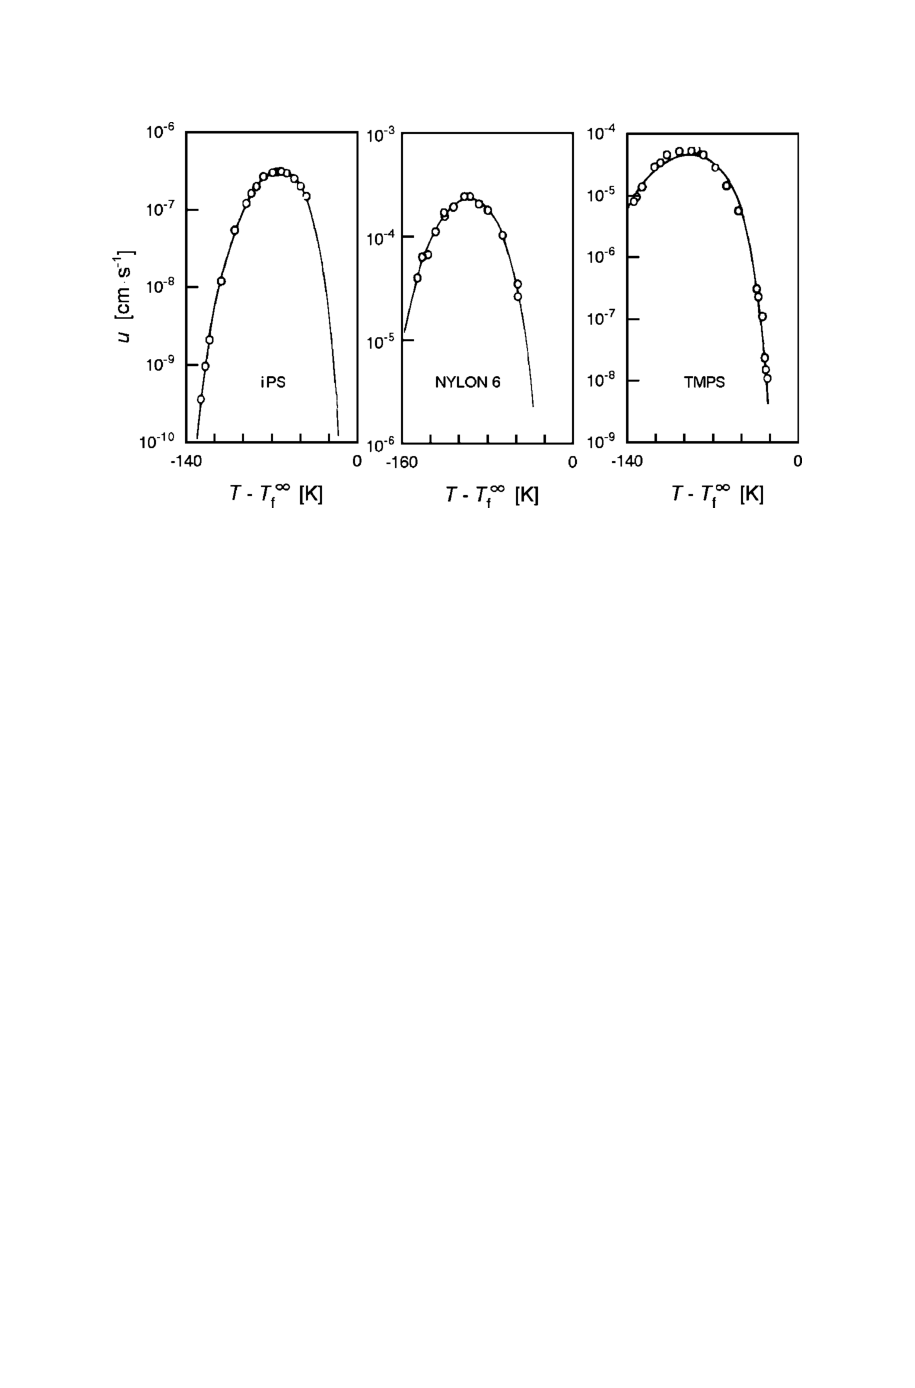
\includegraphics[width=\linewidth]{GvsT}
\caption[Temperature dependence of the radial growth rate $u$ of spherulites of iPS, nylon and TMPS.]{Temperature dependence of the radial growth rate $u$ of spherulites of iPS, nylon and TMPS \cite{Ross1980}.}
\label{fig:growth rate vs T}
\end{figure}


%Crystallinity (437A deleted)

%Crystallinity is defined as the volume fraction of crystalline part in a sample. As polymer liquid turns into crystal, its crystallinity can be modeled using Avrami equation (Avrami, 1939). In deriving this equation, some assumptions are made: nucleation is random and homogeneous across the sample; the growth rate is constant and is the same in all directions, which means the nuclei are spherical. (Jena & Chaturvedi, 1992) Define I0 as the nucleation rate per unit volume, and G as the growth rate. Since crystallization can only take place in liquid, the volume of crystallized material needs to be excluded. However, to simplify the calculation, first take the entire sample as liquid. From time τ to τ+dτ, where 0<τ<t, the number of nuclei formed is
%N=VI_0 dτ.
%Since the radius of a nucleus r is G(t-τ), the crystallized volume is given by
%dV_c^'=4π/3 G^3 〖(t-τ)〗^3 VI_0 dτ.
%Integrating from 0 to t leads to
%V_c^'=π/3 VI_0 G^3 t^4.
%As a matter of fact, the volume of previously crystallized material needs to be excluded. The real volume is
%dV_c=1-V_c/V dV_c'.
%Therefore 
%dV_c^'=1/(1-V_c/V) dV_c.
%By integration, 
%ln⁡(1-Y)=-(V_c^')/V=-π/3 I_0 G^3 t^4,
%where Y=V_c/V is the relative crystallinity. Thus 
%1-Y=exp⁡(-π/3 I_0 G^3 t^4).
%The general form of Avrami equation is given by 
%Y=1-exp⁡(-Kt^n).
%In this special case, K=π/3 I_0 G^3, and n=4.

\section{Review of PEO oligomers crystal growth rate}

Crystal growth rate of PEO oligomers, the material in our case, has been investigated by many researchers. One of the earliest and most famous study was done by Kovacs \textit{et al} \cite{Kovacs1975}. Figure \ref{fig:Kovacs} shows the growth rates vs temperature and molecular weight.

\begin{figure}[H]
\center
\vspace{1 cm}
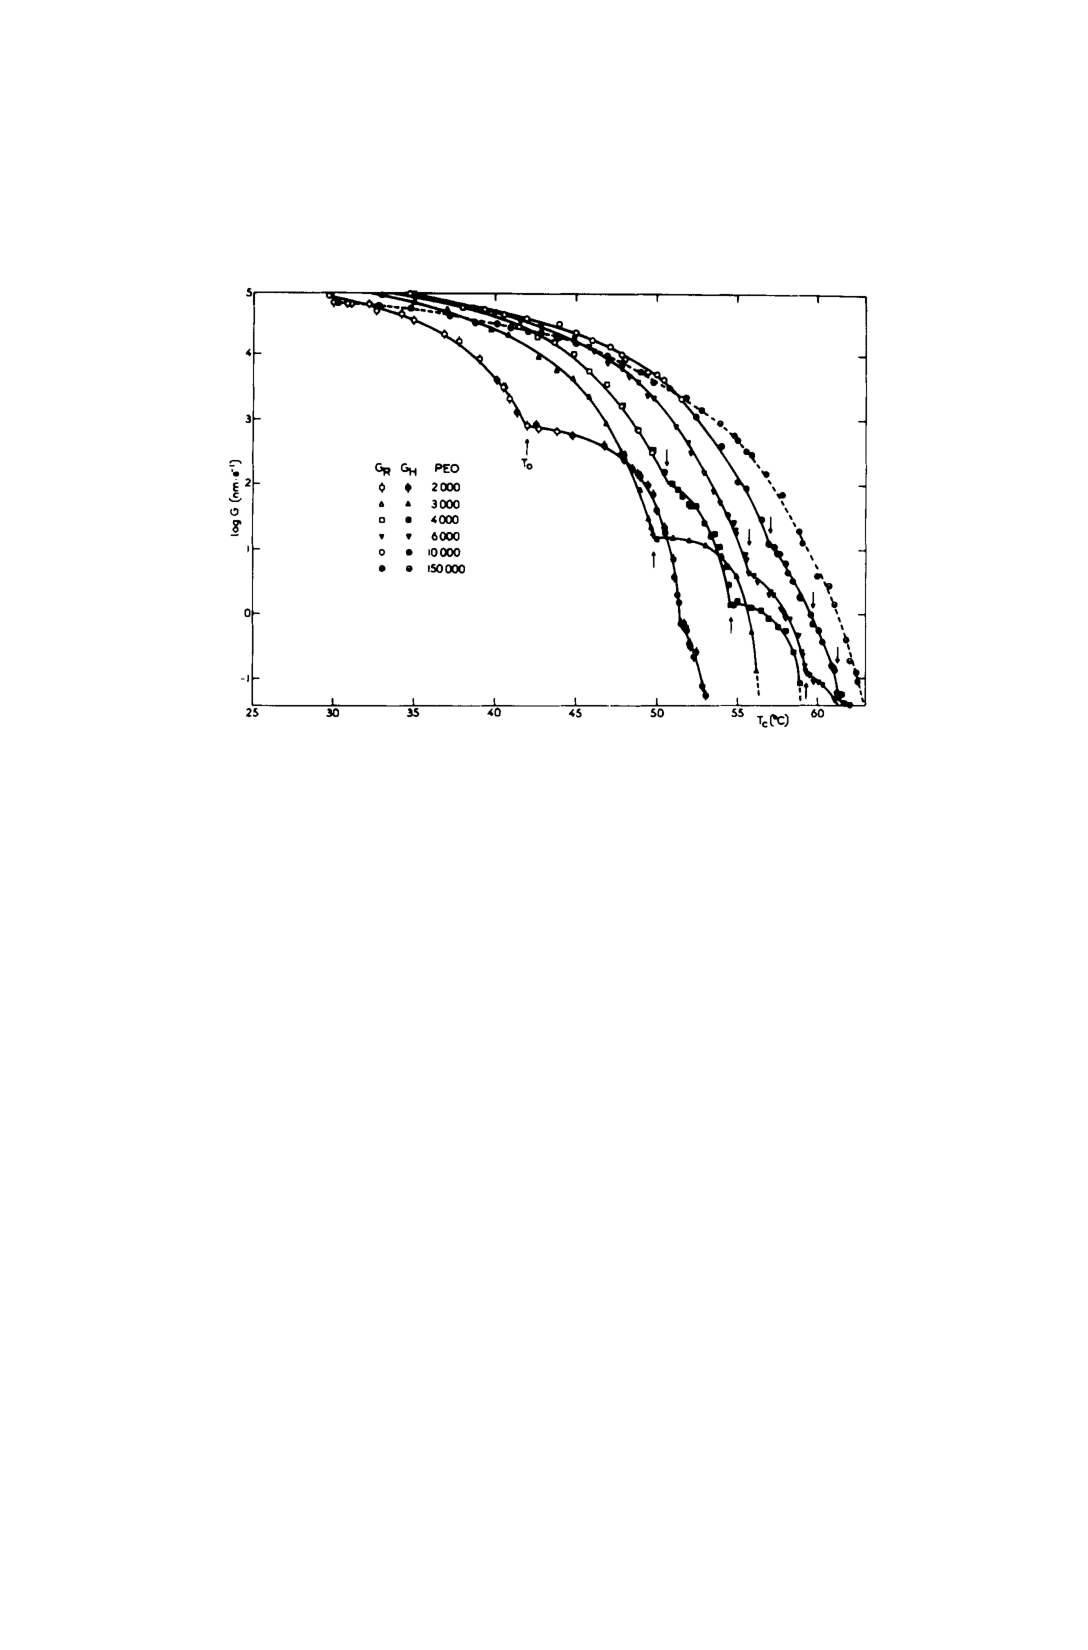
\includegraphics[width=\linewidth]{Kovacs}
\caption[PEO crystals growth rate with respect to temperature and molecular weight.]{PEO crystals growth rate with respect to temperature and molecular weight \cite{Kovacs1975}.}
\label{fig:Kovacs}
\end{figure}

Two types of growth rates were measured in this study. $G_{R}$ refers to the radial growth rate of spherulites, and $G_{H}$, or $G(010)$, refers to the radial growth rate along (010) prism faces. For the measurement of $G_{R}$, several low molecular weight PEO were sandwiched between cover slips, forming films about \SI{10}{\micro\metre}, and crystallized under different temperatures. The growth rates of spherulites were directly measured under optical microscope with crossed polarizers. For the measurement of $G_{H}$, PEO single crystals were grown from thin molten films with thickness about 100 nm, and examined by an electron microscope.

Five low molecular weight samples and one high molecular weight sample were investigated, and from the figure it is seen that $G_{R}$ and $G_{H}$ data agree perfectly with each other, showing no significant difference. Both growth rates expand over six orders of magnitudes, and they could be considered to belong to the higher temperature half in Figure \ref{fig:growth rate vs T}, where the growth rate slows down as supercooling decreases. Along the curve of each low molecular weight, there is as least one sharp transition point. These points are believed to be transition temperatures $T(n)$, where the polymer chains in the crystal turn from $n$-times fold to $(n+1)$-times fold. The high molecular weight curve does not display such a transition point.

\section{Optical microscopy experiments}

With our purified products of PEO oligomers, we also did measurements on crystal growth rates under optical microscope with crossed polarizers. With each sample, we watch crystallization, take a series of pictures with fixed time intervals, as shown in Figure \ref{fig:growth}, and measure the radius of a spherulite in each picture. A graph of crystal size as a function of crystallization time is then generated (Figure \ref{fig:crystal size}), and the growth rate is calculated from the slope of the graph. This process is repeated at different crystallization temperatures, and with fractions having different $\bar{N}$ values.

\begin{figure}[H]
\center
\vspace{1 cm}
\includegraphics[width=0.8\linewidth]{growth}
\caption{Four sequential images of fraction with $\bar{N} = 12.4$ at 260.65 K, under optical microscope with crossed polarizers on.}
\label{fig:growth}
\end{figure}

\begin{figure}[H]
	\center
	\vspace{1 cm}
	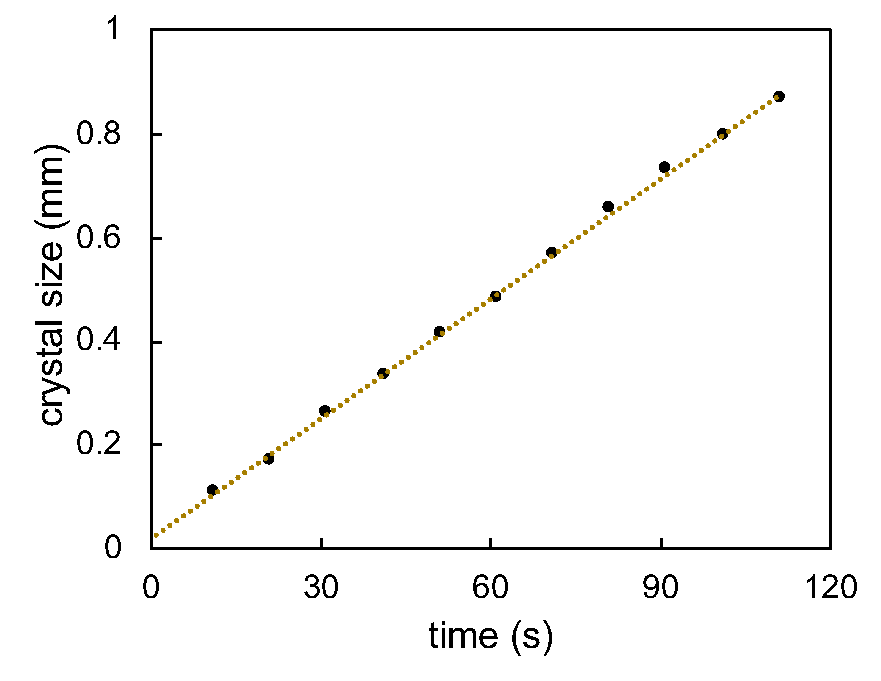
\includegraphics[width=0.6\linewidth]{crystalsize}
	\caption{Crystal size as a function of crystallization time, of fraction with $\bar{N} = 12.4$ at 260.65 K.}
	\label{fig:crystal size}
\end{figure}

\section{Crystal growth rate of purified products}

We performed growth rate measurements with four of our fractions, and the results are shown in Figure \ref{fig:logGvsTc}.

\begin{figure}[H]
	\center
	\vspace{1 cm}
	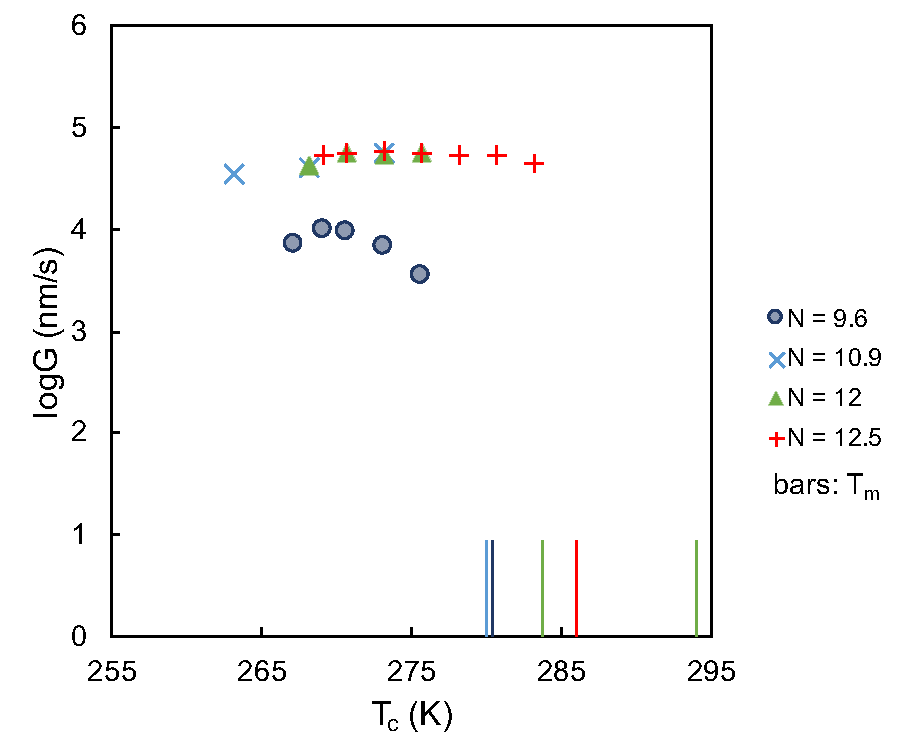
\includegraphics[width=0.8\linewidth]{logGvsTc}
	\caption{Crystal growth rate vs crystallization temperature, with four fractions having different chain lengths. Vertical bars are the melting temperatures of the fractions.}
	\label{fig:logGvsTc}
\end{figure}

At low enough temperatures, the supercooling is large, so we observe fast nucleation process, fast crystal growth, and sufficiently bright contrast. However, at temperatures closer to $T_{m}$, the driving force becomes small due to small supercooling, which results in very difficult nucleation, and the contrast from the crystal is weak so that growth rate could not be measured successfully. Therefore, we have obtained data only for low crystallization temperatures and large growth rates. By looking at the graph itself, we could not find a clear trend, but when we compare it with Figure \ref{fig:Kovacs}, it could be seen that our data agrees with the low temperature plateau regions in terms of scale in their study. In order to get the full picture of crystal grow of our samples, improvements in experiments are still required so that we could be able to measure crystallization under small supercoolings, and reach the rapid decreasing regions.

\chapter{Conclusion \& discussion}

To conclude, the three chapters in the main body are the three major investigations conducted with oligomeric PEO: evaporative purification, chain-conformation, and crystal growth. We applied the evaporative purification technique to obtain highly monodisperse PEO oligomers. The purified products have been examined with mass spectroscopy, in order to characterize the distribution of N’s. With DSC, we studied their crystallization and melting behaviors.

\section{Evaporative purification of PEO}

Through evaporative purification, the distribution of purified samples gets significantly narrowed down compared to that of the neat sample. Quantitatively the polydispersity is approximately six time better, according to the MALDI results. The evolution curves of different $N$ values intuitively show that specific distribution of $N$’s could be assigned correspondingly to the evaporation time or temperature, which provides the possibility of commercializing this purification technique for low molecular weight polymers. In order to further reduce PDI, some practical improvements include: applying larger scale of neat sample; reducing collection intervals; carrying out multiple cycles of evaporation. As a matter of fact, PEO is not a perfect material in terms of this evaporation technique, as the vapor pressures of different $N$ values are not well separated. Comparing to those of polystyrene \cite{Zhu2017a}, the gaps between each two vapor pressure curves of PEO are smaller, which results in more difficult separation through evaporation.

\section{Chain conformation}

The full extended length of the largest $N$ we obtained ($N$ = 16) is less than 5 nm, while polymer crystal lamella is commonly on the order of 10 nm in thickness \cite{Savage2015}. Although the $N$ values we have obtained are still considered small, and normally not expected to be able to fold, the best model to describe our $T_{m}$ data from DSC measurements is that the higher $T_{m}$’s adopt the extended chain mode, and the lower $T_{m}$’s adopt the once-folded chain mode. Furthermore, the fact that we are able to eliminate the lower $T_{m}$ and generate only the higher $T_{m}$ through thermal treatment proves that we could tune the chain-folding mode from extended chains to once-folded chains, which is a direct validation of our model. For common commercial PEO oligomer samples, PDI is high, and the distribution over different chain lengths is broad, which potentially makes it difficult for all of them to make a once-fold and form an ordered conformation in the lamella. However, when chain lengths are all similar, it is possible that the entropy of a once-folded lamella surface is lower, which makes this conformation easier to exist. The measurement of crystallinity was limited by the instrumentations, and thus a larger scale of evaporation could also benefit crystallinity measurement.

\section{Crystal growth}

Processes, kinetics, and crystal structures in polymer crystal growth are reviewed in Chapter \ref{chap_growth}. Macrostructures named spherulites are formed in polymer crystal growth, and the measurements of PEO crystal growth rates are conducted based on the measurements of spherulite size under an optical microscope. The fact that nucleation rate is much slower than crystal growth rate enables us to conveniently carry out the growth rate measurement independently. Due to the weak contrast at temperatures near $T_{m}$'s, we have only obtained data for PEO crystallization under large supercoolings, which agree well with the data from low temperature regions in the literature. In future work, regions nearer melting temperatures should be examined. In addition, X-ray experiments would also be an ideal way to look further into the crystal lamellae.

\singlespacing

% B I B L I O G R A P H Y
% -----------------------

% The following statement selects the style to use for references.  It controls the sort order of the entries in the bibliography and also the formatting for the in-text labels.
%\bibliographystyle{plain}
\bibliographystyle{unsrt} %(does not show url)
%\bibliographystyle{unsrtnat} %(shows url)
% This specifies the location of the file containing the bibliographic information.  
% It assumes you're using BibTeX (if not, why not?).
\cleardoublepage % This is needed if the book class is used, to place the anchor in the correct page,
                 % because the bibliography will start on its own page.
                 % Use \clearpage instead if the document class uses the "oneside" argument
\phantomsection  % With hyperref package, enables hyperlinking from the table of contents to bibliography             
% The following statement causes the title "References" to be used for the bibliography section:
\renewcommand*{\bibname}{References}

% Add the References to the Table of Contents
\addcontentsline{toc}{chapter}{\textbf{References}}

\bibliography{introduction,evaporation,analysis,growth,conclusion}

% Tip 5: You can create multiple .bib files to organize your references. 
% Just list them all in the \bibliogaphy command, separated by commas (no spaces).

% The following statement causes the specified references to be added to the bibliography% even if they were not 
% cited in the text. The asterisk is a wildcard that causes all entries in the bibliographic database to be included (optional).
\nocite{*}

\end{document}
